%%%%%%%%%%%%%%%%%%%%%%% file template.tex %%%%%%%%%%%%%%%%%%%%%%%%%
%
% This is a general template file for the LaTeX package SVJour3
% for Springer journals.          Springer Heidelberg 2010/09/16
%
% Copy it to a new file with a new name and use it as the basis
% for your article. Delete % signs as needed.
%
% This template includes a few options for different layouts and
% content for various journals. Please consult a previous issue of
% your journal as needed.
%
%%%%%%%%%%%%%%%%%%%%%%%%%%%%%%%%%%%%%%%%%%%%%%%%%%%%%%%%%%%%%%%%%%%
%
% First comes an example EPS file -- just ignore it and
% proceed on the \documentclass line
% your LaTeX will extract the file if required
\begin{filecontents*}{example.eps}
%!PS-Adobe-3.0 EPSF-3.0
%%BoundingBox: 19 19 221 221
%%CreationDate: Mon Sep 29 1997
%%Creator: programmed by hand (JK)
%%EndComments
gsave
newpath
  20 20 moveto
  20 220 lineto
  220 220 lineto
  220 20 lineto
closepath
2 setlinewidth
gsave
  .4 setgray fill
grestore
stroke
grestore
\end{filecontents*}
%
\RequirePackage{fix-cm}
%
%\documentclass{svjour3}                     % onecolumn (standard format)
\documentclass[smallcondensed]{svjour3}     % onecolumn (ditto)
%\documentclass[smallextended]{svjour3}       % onecolumn (second format)
%\documentclass[twocolumn]{svjour3}          % twocolumn
%
\smartqed  % flush right qed marks, e.g. at end of proof
%
%\usepackage{mathptmx}      % use Times fonts if available on your TeX system
\usepackage{newtxtext,newtxmath}      % use Times fonts if available on your TeX system
%
% insert here the call for the packages your document requires
%\usepackage{latexsym}
%
\usepackage{amsmath}
\usepackage{amssymb}
\usepackage{algorithm}
\usepackage{algpseudocode}
\usepackage{pgfplots}
\usepackage{graphicx}
\usepackage{calc}
\usepackage{mathtools}
\usepackage{color}
\usepackage[inline]{enumitem}
\usepackage{float}
\usepackage{xfrac}
\usepackage[hidelinks]{hyperref}
\usepackage[capitalize, noabbrev]{cleveref}
\usepackage{longtable}
\usepackage{booktabs}
\usepackage{xspace}
\usepackage{manfnt}
\usepackage{siunitx}
\usepackage{float}

\usetikzlibrary{matrix}
\usepgfplotslibrary{groupplots}
\newfloat{algorithm}{t}{lop}

\definecolor{tol/contrast/blue}{RGB}{0,68,136}
\definecolor{tol/contrast/red}{RGB}{187,85,102}
\definecolor{tol/contrast/yellow}{RGB}{221,170,51}

\definecolor{tol/vibrant/blue}{RGB}{0,119,187}
\definecolor{tol/vibrant/cyan}{RGB}{51,187,238}
\definecolor{tol/vibrant/teal}{RGB}{0,153,136}
\definecolor{tol/vibrant/orange}{RGB}{238,119,51}
\definecolor{tol/vibrant/red}{RGB}{204,51,17}
\definecolor{tol/vibrant/magenta}{RGB}{238,51,119}
\definecolor{tol/vibrant/grey}{RGB}{187,187,187}

\definecolor{tol/rainbow/26}{RGB}{220,5,12}
\definecolor{tol/rainbow/18}{RGB}{247,240,86}
\definecolor{tol/rainbow/15}{RGB}{78,178,101}
\definecolor{tol/rainbow/10}{RGB}{25,101,176}

% please place your own definitions here and don't use \def but
% \newcommand{}{}

\newcommand{\titletable}[2]{\bgroup\renewcommand{\arraystretch}{1.0}\begin{tabular}{@{}c@{}}{#1}\\\scalebox{0.75}{$N={#2}$}\end{tabular}\egroup}
\renewcommand{\vec}[1]{\boldsymbol{#1}}

\newcommand{\param}{\theta}
\newcommand{\params}{\vec{\theta}}
\newcommand{\laplacian}{\Delta}
\newcommand{\cross}{\times}
\newcommand{\grad}[1][]{\nabla\if\relax\detokenize{#1}\relax\else{}_{#1}\fi}
\renewcommand{\div}[1][]{\grad[#1]\cdot}
\renewcommand{\d}{\relax\ifnum\lastnodetype>0\mskip\thinmuskip\fi\textnormal{d}}
\renewcommand{\L}{\mathcal{E}}

\newcommand{\domain}{\ensuremath{\Omega}}
\newcommand{\interface}{\ensuremath{\Gamma}}
\newcommand{\archetype}{\ensuremath{\hat{\Gamma}}}
\newcommand{\reference}{\ensuremath{\interface_0}}
\newcommand{\spread}{\ensuremath{\mathcal{S}}}
\newcommand{\interp}{\ensuremath{\mathcal{S}^\dagger}}
\newcommand{\Dirac}{\delta}
\newcommand{\kernel}{\phi}
\newcommand{\basic}{\varphi}
\newcommand{\Basic}{\Phi}
\newcommand{\poly}{p}
\newcommand{\Poly}{P}

\newcommand{\x}{\vec{x}}
\newcommand{\X}{\vec{X}}
\renewcommand{\u}{\vec{u}}
\newcommand{\U}{\dot{\vec{X}}}
\newcommand{\f}{\vec{f}}
\newcommand{\F}{\vec{F}}
\newcommand{\um}{\mskip\thinmuskip\si{\micro\meter}}

% Insert the name of "your journal" with
% \journalname{myjournal}
\journalname{Journal of Scientific Computing}
%
\begin{document}

\title{%
    A fine-grained parallelization of the immersed boundary method
    %\thanks{$thanks$}
}

%\subtitle{}
%\titlerunning{}

\author{Andrew Kassen \and Varun Shankar \and Aaron Fogelson}

\authorrunning{}
%\authorrunning{Short form of author list} % if too long for running head

\institute{%
    A. Kassen \at Department of Mathematics \newline University of Utah \and
    V. Shankar \at School of Computing \newline University of Utah \and
    A. Fogelson \at Department of Mathematics \newline University of Utah \newline
    \email{fogelson@math.utah.edu}
}

\date{Received: date / Accepted: date}
% The correct dates will be entered by the editor


\maketitle

\begin{abstract}
    This note describes a parallel implementation of the immersed
    boundary method which relies on the well-studied parallel primitives
    key-value sort and segmented reduce. This makes the algorithms feasible for
    use on general purpose graphical processing units in addition to most other
    architectures. This is compared to existing parallelization methods.

% \keywords{}
% \PACS{}
% \subclass{MSC code1 \and MSC code2 \and more}
\end{abstract}

\section{Introduction}

Many problems in biophysics involve the interaction of an incompressible fluid and an
immersed elastic interface. The solution to these problems can be approximated using the
immersed boundary (IB) method, which was developed by Charles Peskin to simulate blood
flow through the heart \cite{Peskin:1972wa}. The relative ease by which the IB method can
be incorporated into a Navier-Stokes solver has led to its popularity in myriad
applications (see, e.g. \cite{Iaccarino:2005ii,Griffith:2020hi} and references therein).
The IB method couples the equations governing fluid velocity and pressure to those
governing the interface movement and elastic forces via operations we will refer to as
\term{interpolation} and \term{spreading}. Fluid velocities are interpolated to points on
the interface, and forces on the interface are spread to the fluid. Fluid properties are
discretized on a fixed Eulerian grid. The interface is represented by a set of mobile
Lagrangian points. This presents a problem for effective parallelization of interpolation
and spreading, as these operators must be reconstructed at each timestep to account for
the motion of the Lagrangian points relative to the Eulerian grid. The Eulerian and
Lagrangian points, on the other hand, can be treated as fixed in their respective
coordinate spaces for several timesteps, if not for the entirety of a simulation. We may
therefore treat solving the fluid equations and computing elastic forces as an
implementation detail and focus primarily on the interpolation and spreading operations.

We are interested in the case of neutrally buoyant, elastic immersed structures that move
at the local fluid velocity, but do not impose it. In particular, we aim to simulate
whole blood, which is composed of red blood cells (RBCs) and platelets immersed in blood
plasma, within a vessel lined by endothelial cells. The cells are elastic, and as they
deform with the flow of the enveloping fluid, impose a force on the fluid.  Approximately
40\% of the volume in healthy human blood is occupied by RBCs, and so even small domains
may require tens or hundreds of thousands of points to discretize these cells for use
within the IB method.

To take advantage of modern computing architectures, with ever-increasing numbers of
processors, it is necessary to develop parallel algorithms for the IB method.
McQueen and Peskin \cite{McQueen:1997kw} present a domain decomposition scheme to
parallelize the interpolation and spreading operations on the Cray C-90 computer with
shared memory and a modest number of vector processors. Their results illustrate the need
for a fast interpolation and spreading: even parallelized, they spend roughly half of the
wall clock time spreading and interpolating. Fai, \textit{et al.} \cite{Fai:2013do}
adapted this domain decomposition scheme for use on a general purpose graphical
processing unit (GPGPU; GPU for short). Patel \cite{Patel:2012tc} parallelized spreading
on a GPU by processing one Lagrangian point at a time. Because neither of these
approaches can concurrently process arbitrary Lagrangian points, it is easy to find cases
for which they perform poorly. An alternative is to distribute work among several
devices, each with its own memory. This idea underpins the popular IBAMR library
\cite{Griffith:2007uk,Griffith:2007do,Griffith:2009gg, Griffith:2011gi, Griffith:2017id},
which also adaptively refines the mesh around the immersed structure. With proper
load-balancing, this allows a serial algorithm to process a smaller portion of work.
A cluster of multicore devices, however, will not be used effectively without a
shared-memory parallel algorithm. The cuIBM \cite{Layton:2011um} and PetIBM
\cite{Mesnard:2017te,Chuang:2018ej} libraries implement an adaptive IB method for
prescribed motion on single- and multi-GPU architectures, respectively. The authors
demonstrate their method on a few two-dimensional test problems. Their implementation
explicitly construct the spreading and interpolation operators, which are sparse, but the
sparsity pattern of the spreading matrix does not always lend itself well to
parallelization.

GPUs have restrictions on their parallelization. They use single instruction,
multiple data (SIMD) parallelism, in which each computational unit, or thread, executes
the same instruction on its own data. Concurrency on the GPU is typically limited by the
amount of shared memory, which is shared among a group of threads, and register memory, which is
accessible only to a single thread. The alternative is to use global memory, which is
slow in general, but faster when accesses are sequential (or ``coalesced''). These
restrictions on the GPU imply that an effective algorithm for the GPU translates well to
other shared-memory architectures, such such as multicore CPUs, which support
parallelism, SIMD instructions, advanced instruction pipelining, and out-of-order
execution. We therefore develop parallel spreading and interpolation algorithms
applicable to both GPUs and multicore CPUs. The success of our new algorithms relies in
dividing these operations into trivially parallelizable tasks and parallel primitives.

The remainder of this paper is organized into four sections. Section \ref{sec:ib} gives
an overview of the IB method, and describes the role of the interpolation and spread
operations. In Section \ref{sec:parallel}, we discuss the parallelization of
interpolation and introduce a new parallelization for the spreading operation. In Section
\ref{sec:results}, we demonstrate that the concurrency of these algorithms scales with
the number of IB points, independently of the Eulerian grid. We confirm the convergence
of the IB method with these new algorithms. We illustrate the suitability of our
algorithms to both GPUs and multicore CPU architectures with both weak and strong scaling
tests. Finally, we summarize our findings in Section \ref{sec:summary}.

% vim: cc=90 tw=89

\section{Review of the immersed boundary method}

Consider a $d$-dimensional ($d=2$ or 3) rectangular domain $\domain$, which is filled
with a viscous incompressible fluid with constant viscosity $\mu$ and density $\rho$, and
contains an immersed elastic structure, $\interface$. The structure is impermeable to the
fluid and moves at the local fluid velocity, is deformed by this motion, and imparts a
force to the fluid. Otherwise, the interface is treated as part of the fluid. 

The fluid velocity, $\u = \u(\x,\,t)$, and pressure, $p = p(\x,\,t)$, are governed by the
incompressible Navier-Stokes equations for a Newtonian fluid,
\begin{gather}
    \label{eq:ins-evol}
    \rho(\u_t + \u\cdot\grad\u) = \mu\Delta\u - \grad p + \f, \\
    \label{eq:ins-incomp}
    \div\u = 0,
\end{gather}
where $p$ is the pressure and $\f$ is the elastic force density. This is a set of $d+1$
equations in $d+1$ unknowns: the $d$ components of $\u$, and $p$. The equations are
written relative to the Eulerian frame, so that the coordinates $\x$ are independent
variables. Throughout, we write Eulerian quantities in the lowercase Latin alphabet.

Let $\X=\X(\params,\,t)$ represent a parametrization of the Cartesian coordinates of the
immersed interface with material coordinates $\params$ at time $t$. Let $\L[\X]$ be the
energy density functional for the elastic interface material. The elastic force density
is computed by evaluating the Fréchet derivative of $\L$,
\begin{equation}
    \label{eq:forces}
    \F = -\delta \L[\X],
\end{equation}
where $\delta$ represents the first variation. Uppercase Latin letters represent
Lagrangian quantities and are functions of $\params$ and $t$.

The interface moves at the local fluid velocity, and force balance on the interface
between the interface and fluid dictates that the interface force on the fluid is equal
to the elastic force. Analytically, the fluid-interface interactions can be written
\begin{gather}
    \label{eq:interpolation}
    \U(\params,\,t) = \int_\domain \Dirac(\x-\X(\params,\,t)) \u(\x,\,t)\d\x,\ \text{and} \\
    \label{eq:spreading}
    \f(\x,\,t) = \int_\interface \Dirac(\x-\X(\params,\,t))\F(\params,\,t)\d\params,
\end{gather}
where $\U(\params,\,t)$ represents the derivative of $\X(\params,\,t)$ with respect to
$t$, and $\Dirac(\x-\X(\params,\,t))$ is the Dirac $\Dirac$-function centered at
$\X(\params,\,t)$.  Equation \eqref{eq:interpolation} is called \term{interpolation}, and
the result of the right-hand side is the fluid velocity at $\X(\params,\,t)$; namely,
$\U(\params,\,t) = \u(\X(\params,\,t),\,t)$.  Equation \eqref{eq:spreading} is called
\term{spreading}, because while $\F(\params,\,t)$ has units of force per unit \emph{area}
on $\interface$, $\f(\x,\,t)$ has units of force per unit \emph{volume} in $\domain$. The
force $\F(\params,\,t)\d\params$ over area $\d\params$ is ``spread'' to the force
$\f(\x,\,t)\d\x$ over volume $\d\x$. 

Each of the fluid equations \eqref{eq:ins-evol}--\eqref{eq:ins-incomp}
is discretized on a regular grid of spacing $h$ so that $\domain$ is divided into square
or cubic cells of side length $h$. Because of the checkerboard instability (see, e.g.,
\cite{Wesseling:2001ci}) in solving the Navier-Stokes equations on collocated regular
grids, we stagger the components of Eulerian vector quantities. As a result, different
components are discretized at different locations, but corresponding components are
discretized on the same grid. Grid cells for these staggered grids do not coincide. We
therefore consider each of these grids individually. We use $\domain_h$ to denote the set
of grid points for the grid under consideration, and $n_\omega$ to denote the number of
grid points.

The Lagrangian force density \ref{eq:forces} is evaluated at a set of points, usually a
\emph{fixed} set of points in material coordinates, referred to as IB points. The
notation $\X_j=\X(\params_j,\,t)$ refers to an individual IB point on $\interface$ in
Cartesian coordinates. The typical heuristic for distributing the points $\X_j$ on the
interface places neighboring IB points at most $h$ apart from one another, and often at
most $h/2$ apart. We therefore denote the set of IB points by $\interface_h$ and the
number of IB points by $n_\gamma$.

The singular integrals \eqref{eq:interpolation} and \eqref{eq:spreading} do not lend
themselves easily to evaluation. In particular, it is unlikely that IB points and grid
points will coincide. For a regular grid with spacing $h$, we replace the Dirac
$\Dirac$-function with a regularized kernel, $\Dirac_h$, which is a product of
one-dimensional kernels, $h^{-1}\kernel(h^{-1}x)$. There are several options for
$\kernel$ \cite{Griffith:2020hi}, but we will restrict ourselves to the simple cosine
kernel \cite{Peskin:2002go}.

Let $\domain_h$ be one of the Eulerian grids for vector-valued quantities. Discretizing
equations \eqref{eq:scalar-interp} and \eqref{eq:scalar-spread} on $\domain_h$ and
$\interface_h$, respectively, yields
\begin{align}
    \label{eq:disc-interp}
    \dot{X}^n_j &= \sum_i \delta_h(\x_i-\X^n_j)u^n_i h^d \quad \text{and} \\
    \label{eq:disc-spread}
    f^n_i &= -\sum_j \delta_h(\x_i-\X^n_j)F^n_j \d\theta_j,
\end{align}
where $u^n_i$ and $f^n_i$ are discrete approximations to the components of $\u$ and $\f$
at $\x_i\in\domain_h$ and time $t=t_n$, and $\dot{X}^n_{\smash j}$ and $F^n_{\smash j}$
are their Lagrangian counterparts at $\X_{\smash j}$, respectively. The terms $h^d$ and
$\d\theta_{\smash j}$ are integration weights analogous to $\d\x$ and $\d\params$. Each
of the above equations look like a matrix-vector multiplication, so we define the
\emph{spreading matrix} $\spread=(\delta_h(\x_i-\X^n_{\smash j}))$ with row $i$ and
column $j$. We call its transpose, $\interp$, the \emph{interpolation matrix}. Collecting
values $u^n_ih^d$ as $\u^n$ at each grid point and $F^n_{\smash j}\d\theta_{\smash j}$ as
$\F^n$ at each IB point, we rewrite Equations \eqref{eq:disc-interp} and
\eqref{eq:disc-spread} in matrix form as
\begin{align}
    \label{eq:matrix-interp}
    \dot{\X}^n &= \interp\u^n \quad\text{and} \\
    \label{eq:matrix-spread}
    \f^n &= \spread\F^n,
\end{align}
respectively.

Collectively, the equations \eqref{eq:ins-evol}--\eqref{eq:spreading} constitute the
IB method, and while different implementations depend on myriad details, a single step
proceeds with timestep $k$ roughly as follows:
\begin{enumerate}[label=(\texttt{\alph*})]
    \item interpolate $\u^n$ to $\X^n$ to get $\U^\ast$,
    \item predict Lagrangian positions $\X^\ast = \X^n + k\U^\ast$,
    \item compute Lagrangian forces $\F^\ast$ using positions $\X^\ast$,
    \item spread $-\F^\ast$ from $\X^\ast$ to get $\f^\ast$,
    \item solve for updated Eulerian velocities $\u^\ast$,
    \item project $\u^\ast$ into space of divergence-free vector fields to get
        $\u^{n+1}$,
    \item interpolate $\u^{n+1}$ to $\X^n$ to get $\U^{n+1}$, and
    \item update $\X^{n+1} = \X^n + k \U^{n+1}$.
\end{enumerate}
We group these steps into 3 categories: the purely Eulerian (\texttt{e}) and
(\texttt{f}); the purely Lagrangian (\texttt{b}), (\texttt{c}), and (\texttt{h}); and the
Eulerian-Lagrangian coupling (\texttt{a}), (\texttt{d}), and (\texttt{g}). We discuss the
%parallelization of the
first two categories \textcolor{red}{in a forthcoming paper}.
%
%briefly before tackling the third.
%
%\section{Parallelization in the Eulerian and Lagrangian frames}
%
%Given an Eulerian force density $\f$ and Lagrangian fluid velocity $\U$ it is
%a straightforward matter to parallelize the evolution of the fluid velocity and interface
%forces, as they are otherwise independent of one another. Assuming fixed sets of grid
%points and material coordinates for IB points, any interdependence of points within a
%frame can be accounted for at the outset to ease parallelization during the course of a
%simulation.
%
%To solve for the fluid velocity, we use the 2nd-order Runge-Kutta method described in
%\cite{Peskin:2002go}.  We compute the advection term in conservation form. For, e.g., the
%quantity $(uv)_y$, we average $u$ in the $y$ direction and $v$ in the $x$ direction. The
%product of these averages is then differentiated in the $y$ direction. We correct near
%boundaries to ensure exact recovery of parabolic flows. This involves scaling certain
%terms by a constant factor to account for errors in discretizing the Laplacian near the
%boundary. To take advantage of the GPU, the solver must be highly parallel. To that end,
%the Helmholtz equations that arise from discretizing equation \eqref{eq:ins-evol} are
%solved using conjugate gradients preconditioned with Chebyshev iteration. Chebyshev
%iteration is an attractive method because, other than parallel vector addition and
%scaling, it requires only the ability to perform sparse matrix-vector multiplication.
%This can be achieved with the appropriate sparse storage formate and a linear algebra
%library such as Intel's \texttt{MKL} or NVIDIA's \texttt{cuSPARSE}. Incompressibility is
%enforced using PmIII of \cite{Brown:2001bq}.  Satisfying the incompressibility condition
%\eqref{eq:ins-incomp} requires a Poisson solve, which is done using conjugate gradients
%preconditioned with full-weighting multigrid. The multigrid routine also uses Chebyshev
%iteration, restricted to high-frequency modes, for relaxation. The resulting solver is
%highly parallel and is suitable for any combination of boundary conditions.
%
%Elastic structures are modeled using radial basis functions (RBFs) to construct the
%surface, as in \cite{Shankar:2015km}. The Fr\'echet derivative in equation
%\eqref{eq:forces} is computed analytically, following \cite{Maxian:2018ek}, and evaluated
%by computing tangents and higher-order surface derivatives on the structure. These
%differential operators are dense, but computed only once and used throughout the course
%of a simulation. The forces are used in equation \eqref{eq:spreading}, for which we
%require integration weights. As the structures of interest are topologically spheres, we
%follow \cite{Fuselier:2013coba} to compute weights on the sphere, and geometric
%information about both the sphere and the structure to obtain appropriate weights for the
%structure \cite{Maxian:2018ek}. The construction of the operators and their application
%requires a way to solve linear systems and perform dense matrix-matrix and matrix-vector
%multiplications. The \texttt{LAPACK} and \texttt{BLAS} libraries are the standard. There
%are numerous parallel implementations of these libraries; for the GPU, we employ NVIDIA's
%implementations, \texttt{cuSOLVER} and \texttt{cuBLAS}.
%
%The interaction operations, however, must take into account the motion of the Eulerian
%and Lagrangian frames relative to one another, and must therefore be recomputed every
%timestep. The remainder of this paper discusses the implementation and parallelization
%of these operations.
The remainder of this paper discusses the implementation and parallelization of the
third.

% vim: cc=90 tw=89

\section{Fluid solver}

\subsection{Spatial discretization}

The equations [@eq:...] are discretized on staggered, regular grids with grid
spacing $h$. The components of vector-valued quantities are discretized on the
center of the corresponding cell face. That is, for example, if
$\vec{a} = (a_1,\,a_2,\,a_3)$ are the three components of a vector-valued
quantity for some grid cell with lower corner $h(i,\,j,\,k)$, then $a_1$
lives at $h(i,\,j+0.5,\,k+0.5)$, $a_2$ at $h(i+0.5,\,j,\,k+0.5)$, and $a_3$ at
$h(i+0.5,\,j+0.5,\,k)$. Scalar quantities are discretized at cell centers,
e.g., $h(i+0.5,\,j+0.5,\,k+0.5)$.

The central difference operator $D_i$, which differentiates with respect to
the $i^\text{th}$ coordinate, in the absence of solid boundaries, is defined as
\begin{equation}
    D_ig(\vec{x}) = \frac{g(\vec{x}+h\vec{e}_i/2) + g(\vec{x}+h\vec{e}_i/2)}{h}.
\end{equation}
In the presence of solid boundaries, a linear interpolant is used to fill a
ghost value. The divergence operator applied to a vector-valued function
$\vec{a}$ on the staggered grid, $\grad_h\cdot\vec{a} = D_ia^i$, where Einstein
summation notation is assumed and $i$ ranges from 1 to $d$, results in
a scalar-valued quantity at the cell center. The gradient operator applied to
scalar-valued quantity $b$ at the cell center yields the vector
$\grad_hb = \vec{e}^jD_jb$ on the staggered grid.

Define the central averaging operator, $A^i$, which averages in the
$i^\text{th}$ coordinate direction and in the absence of boundaries, as
\begin{equation}
    A_i = \frac{g(\vec{x}+h\vec{e}_i)+g(\vec{x}-h\vec{e}_i)}{2}.
\end{equation}
In the presence of boundaries, we use the value at the ghost cell. By taking
products of averaged components of $\vec{u}$, we compute advection in
conservation form as
\begin{equation}
    \vec{H}(\vec{u}) := \vec{e}_iD_j((\delta^{im}A_mu^j)(\delta^{jn}A_nu^i)).
\end{equation}

The viscous terms are computed as $\mu\Delta_h\vec{u}$, where $\Delta_h$ is the
standard 5- or 7-point Laplacian. In the absence of solid boundaries, this
is identical to  $\Delta_h = \grad_h\cdot\grad_h$. Otherwise, we use the value
at the ghost cell for stencils that extend past a solid boundary.

\subsection{Temporal discretization}

We time-step using the 2$^\text{nd}$ order implicit-explicit Runge-Kutta method
as described in [@Peskin:...] and projection method PmIII from [@Brown:...].
This leads to the system of equations
\begin{align}
    \left(\tilde{I}-\frac{\lambda}2\Delta_h\right)\delta\vec{w}
    &= \alpha\lambda\left[\Delta_h\vec{u}^n + B_h \vec{w}_b^{n+\sfrac12}\right] + \tilde{I}\left(\rho^{-1}\vec{f} - \vec{H}(\vec{u}^{n+\alpha-\sfrac12})\right) \\
    \vec{w} &= \vec{u}^n + \delta\vec{w} \\
    k\Delta_h\phi &= \grad_h\cdot\vec{w} \\
    \vec{u}^{n+\alpha} &= \vec{w} - k\grad_h\phi,
\end{align}
where $k$ is the timestep, $\lambda = k\mu/\rho$, $B_h$ is an appropriate
boundary operator for the discrete Laplacian, $\vec{w}_b$ are boundary data for
$\vec{w}$, and $\alpha$ is the fraction of the timestep for the current stage
of the timestepping method: $\alpha=\sfrac12$ or 1. The quantity $\phi$ acts as
a pseudo-pressure, and the pressure can be recovered via
$p=\phi-(\mu/\rho)\grad_h\cdot\vec{w}$.

The modified identity matrix, $\tilde{I}$, corrects errors in using the
standard discrete Laplacian on a staggered grid, where the stencil may extend
beyond the boundary of the domain. This requires a ghost point, to which we
have assigned a value using a linear interpolant. Under certain circumstances,
this works perfectly fine, but in general, the resulting approximation to the
Laplacian is 0$^\text{th}$ order, but differs by a constant factor. Let that
factor be denoted $1-\epsilon_h$. For stencils that straddle the boundary, we
modify the momentum equation so that we are instead solving
\begin{equation}
    (1-\epsilon_h)\rho(\vec{u}_t + \grad\cdot(\vec{u}\otimes\vec{u})) = (1-\epsilon_h)\left[\mu\Delta\vec{u} + \vec{f}\right].
\end{equation}
This requires no additional modification to the Laplacian, but after
discretization, yields a factor in front of the intermediate velocity update
$\delta\vec{w}$ and the force density and advection terms. Under reasonable
assumptions, the resulting linear system is symmetric positive definite, and
is suitable for use with preconditioned conjugate gradients. One can view this
as using a quadratic interpolant near the boundaries and scaling the
corresponding rows to ensure symmetry of the linear system. The resulting
systems are identical.

\subsection{Helmholtz solver}

To solve the Helmholtz system $\tilde{I}-\sfrac12\lambda\Delta_h$, we use
conjugate gradients preconditioned with Chebyshev iteration. Chebyshev
iteration requires only that the matrix be positive (negative) semi-definite,
and uses only matrix-vector multiplication and vector scaling, it is
parallelizable if those two operations are. Vector scaling is trivially
parallelilzable, and for certain matrix formats, such as compressed sparse row,
matrix-vector multiplication is parallelizable as well.

\subsection{Poisson solver}

Chebyshev iteration can also be modified for use as a smoother/relaxer for
multigrid. Its efficacy is comparable or better to that of successive
over-relaxation (SOR), but the parallelism of Chebyshev iteration far exceeds
that of SOR. To solve the Poisson problem for $\phi$, we employ multigrid with
a Chebyshev smoother as a preconditioner for conjugate gradients.



\section{Cell modeling}
Details about cell modeling % XXX

\subsection{Composition of whole blood}

\subsection{Computation of Lagrangian forces}

To compute forces for a cell, we follow the analysis of [@Maxian:...]. The
constitutive laws of interest for our purposes are the Skalak tension law,
\begin{equation}
    W_\text{Sk} = \frac{G}{4}(I_1^2-2I_1+2I_2) + \frac{K}{4}I_2^2;
\end{equation}
the neo-Hookean tension model,
\begin{equation}
    W_\text{nH} = \frac{G}{2}\left(\frac{I_1+2}{\sqrt{I_2+1}}-1\right) + \frac{K}{2}\left(\sqrt{I_1+1}-1\right)^2;
\end{equation}
Hookean tether energy,
\begin{equation}
    W_\text{tether} = \frac{k}{2}\|\vec{X}-\vec{Z}\|^2;
\end{equation}
and the Canham-Helfrich bending energy,
\begin{equation}
    W_\text{CH} = \frac{\kappa}{2}(H-H_0)^2.
\end{equation}
In the above, $G$, $K$, and $\kappa$ are the shear, bulk, and bending moduli,
respectively; $k$ is the spring constant; and $H_0$ is the preferred mean
curvature of the surface.

For each of these, we can compute analytically the force density by directly
computing the first variation of the energy functional
\begin{equation}
    \mathcal{E}[\vec{X}] = \int_\Gamma W\mskip\thinmuskip\mathrm{d}\vec{X}.
\end{equation}
For the Skalak and neo-Hookean tension models, we can rewrite the energy
functional in terms of the undeformed configurations, and write the force
density as
\begin{equation}
    \vec{F} = \frac{1}{\sqrt{\hat{g}}}\frac{\partial}{\partial\theta^j}\left(\sqrt{\hat{g}}\left[\Phi \hat{g}^{ij} + I_2\Psi g^{ij}\right]\frac{\partial\vec{X}}{\partial\theta^i}\right),
\end{equation}
were $\hat{g}^{ij}$ and $\hat{g}$ are the inverse and determinant of the metric
tensor
\begin{equation}
    g_{ij} = \frac{\partial\hat{\vec{X}}}{\partial\theta^i}\cdot\frac{\partial\hat{\vec{X}}}{\partial\theta^j},
\end{equation}
respectively. The inverse metric tensor $g^{ij}$ is the analogue of $\hat{g}^{ij}$
for the deformed configuration. The material functions $\Phi$ and $\Psi$ are
the partial derivatives of the constitutive law, $W$, with respect to $I_1$
and $I_2$, respectively, and the bracketed terms are also known as the
second Piola-Kirchhoff stress tensor. The tether energy yields the tether
force density
\begin{equation}
    \vec{F}_\text{tether} = -k(\vec{X}-\hat{\vec{X}}),
\end{equation}
and the Canham-Helfrich bending energy yields the bending force density
\begin{equation}
\vec{F}_\text{tether} = -\kappa\left[\Delta_{\vec{\theta}}(H-H_0) + (H-H_0)(2H^2-\mathcal{R})\right]\vec{n},
\end{equation}
where, $\mathcal{R}$ is the scalar curvature of the deformed configuration.

\subsection{Topological archetypes}
Sphere and closed surface of genus 1.

\subsection{Surface geometry via radial basis function interpolation}

Fix a set of distinct points $\{\vec{\theta}_i\}_{i=1}^{n_d}$ in parameter
space. We refer to these $n_d$ points as \textit{data sites} and are used to
construct an interpolant which will acts as the surface of a cell. To
accomplish this, we track the coordinates in $\mathbb{R}^3$ of the point on the
surface corresponding to each of the data sites.

We can choose a set of distinct points in parameter space, called the
\textit{sample sites}, which are possibly different from the data sites, at
which to evaluate the interpolant and its derivatives, and ultimately to
compute the Lagrangian force density. These points will be used to spread force
density from the surface to the Eulerian grid, so we choose them to satisfy the
IB method heuristic that the mesh size $h_s$ satisfies $h_s \lesssim h/2$,
where $h$ is the Eulerian grid size.

The surface interpolant is constructed from a linear combination of radial
basis functions and another polynomial basis. While generally, these basis
functions may not be true polynomials, we will refer to them as such for 
simplicity of illustration. Details ... [@Shankar:...].

Let $\vec{X}_k$ be the coordinates of the point on the cell surface
corresponding to data site $\vec{\theta}_k$. The interpolant should recover
these coordinates exactly, for each data site. In other words, we want
\begin{equation}
    \vec{X}_k = \sum_{i=1}^{n_d} b_i\varphi(d(\vec{\theta}_k,\,\vec{\theta}_i)) + \sum_{j=1}^{n_p} c_jp_j(\vec{\theta}_k),
\end{equation}
where $\varphi$ is called the \textit{basic function}, $d$ is a suitable metric
for the object under study, and $n_p$ is the number of elements in the set of
polynomial basis functions $\{p_j\}_{j=1}^{n_p}$. For certain choices of
$\varphi$, $n+p\ge 1$ may be required [@Wendland:...;@Fasshauer:...]. For an
individual component of $\vec{X}$ at each data site, this yields $n_d$
conditions in $n_d+n_p$ variables. To uniquely determine the interpolant, we
require further that the polynomial basis recover polynomial data:
\begin{equation}
    0 = \sum_{i=1}^{n_d} b_ip_j(\vec{\theta}_i).
\end{equation}
Collectively, these conditions can be written
\begin{equation}
    \label{eq:rbf-interpolant}
    \left[\begin{array}{cc}\Phi & P \\ P^T & 0\end{array}\right]
    \left[\begin{array}{c}\vec{b}\\\vec{c}\end{array}\right] =
    \left[\begin{array}{c}\vec{X}\\\vec{0}\end{array}\right].
\end{equation}
Assuming that the system is uniquely determined, we have constructed our
interpolant.

Let $\mathcal{L}$ be a linear operator for which $\Psi=(\mathcal{L}\varphi(d(\vec{\theta},\,\vec{\theta}_i)))$,
for $i=1,\,\ldots,\,n_d$, and $Q=(\mathcal{L}p_j(\vec{\theta}))$, for $j=1,\,\ldots,\,n_p$,
can be computed analytically. For the purposes of computing Lagrangian force
density, of particular interest are the identity (or "evaluation") operator,
and the various first and second partial derivative operators. With
a sufficiently smooth choice of $\varphi$, we can approximate $\mathcal{L}\vec{X}(\vec{\theta})$
at an arbitrary point in parameter space by applying the operator $\mathcal{L}$
to the interpolant and evaluating the result. That is,
\begin{equation}
    \mathcal{L}\vec{X}(\vec{\theta})
    \approx \sum_{i=1}^{n_d} b_i\mathcal{L}\varphi(d(\vec{\theta},\,\vec{\theta}_i))
    + \sum_{j=1}^{n_p} c_j\mathcal{L}p_j(\vec{\theta})
\end{equation}
by linearity. But the coefficients $\vec{b}$ and $\vec{c}$ are determined by
the interpolant [@eq:rbf-interpolant], so
\begin{align}
    \mathcal{L}\vec{X}(\vec{\theta})
    &= \left[\begin{array}{cc}\Psi&Q\end{array}\right]
    \left[\begin{array}{cc}\Phi&P\\P^T&0\end{array}\right]
    \left[\begin{array}{c}\vec{X}\\\vec{0}\end{array}\right] \\
    &= \left[\begin{array}{cc}L&\ast\end{array}\right]
    \left[\begin{array}{c}\vec{X}\\\vec{0}\end{array}\right],
\end{align}
where $L\vec{X}$ is now the discrete analogue to $\mathcal{L}\vec{X}(\vec{\theta})$,
i.e., the operator that applies $\mathcal{L}$ and evaluates at $\vec{\theta}$.
The $n_p$ columns represented by $\ast$ are usually ignored, as they are
always multiplied by a vector of zeros and therefore do not contribute.

We also require integration weights, which act as surface patch areas in
computing surface forces from a surface force density. In many cases, the
integral
\begin{equation}
    I_\varphi(\vec{\theta}') = \int_\Gamma \varphi(d(\vec{\theta},\,\vec{\theta}'))\mskip\thinmuskip\mathrm{d}\hat{\vec{X}}(\vec{\theta})
\end{equation}
may not be known for topological archetype $\Gamma$. But
following the work of [@Narcowitz:...], for certain surfaces,
$I_\varphi(\vec{\theta}')$ is independent of $\vec{\theta}'$ and is therefore
constant. Assuming $I_\varphi = \text{constant}$ and
\begin{equation}
    I_1 = \int_\Gamma \mathrm{d}\hat{\vec{X}}(\vec{\theta})
\end{equation}
is known, we can compute integration weights $\hat{\vec{a}}$ for $\Gamma$ via
\begin{equation}
    \left[\begin{array}{cc}\Phi &\vec{1} \\ \vec{1}^T & 0\end{array}\right]
    \left[\begin{array}{c}\hat{\vec{a}}\\-I_\varphi\end{array}\right] =
    \left[\begin{array}{c}\vec{0}\\I_1\end{array}\right].
\end{equation}
A side effect of solving this system is that we obtain an approximation to
the constant $I_\varphi$.

To compute integration weights for a shape $\vec{X}(\vec{\theta})$, which is
topologically equivalent to $\hat{\Gamma}$, we compute the
Jacobian for $\hat{\Gamma}$ and the cell,
\begin{equation}
    \hat{V}=\left|\frac{\partial\hat{\vec{X}}}{\partial\theta^i}\right| \quad \text{and} \quad
    V=\left|\frac{\partial\vec{X}}{\partial\theta^i}\right|.
\end{equation}
Since $\hat{\Gamma}$ is known, we can compute $\hat{V}$ analytically. The
expression $a_k/\hat{V}(\vec{\theta}_k)$ gives the integration weight in
parameter space and can be computed without any information about the cell,
except that the cell and $\Gamma$ are topologically equivalent. From these
weights and an interpolant for the cell, the expression
$\mathrm{d}A_k=a_k V(\vec{\theta}_k)/\hat{V}(\vec{\theta}_k)$ gives the
integration weight on the surface of the cell.



\section{Parallelization strategies for interpolation and spreading} \label{sec:parallel}

Here, we describe a method for evaluating the discrete counterparts to
\begin{align}
    \label{eq:scalar-interp}
    E(\X) &= \int_\domain \Dirac_h(\x-\X)e(\x) \d\omega \quad \text{and}\\
    \label{eq:scalar-spread}
    \ell(\x) &= \int_\interface \Dirac_h(\x-\X)L(\X) \d\gamma
\end{align}
where scalar-valued Eulerian function $e:\domain\to\mathbb{R}$ is interpolated to
Lagrangian point $\X$ and Lagrangian function $L:\interface\to\mathbb{R}$ is spread to
Eulerian point $\x$. For vector-valued functions, such as the Eulerian fluid velocity
$\u$ and Lagrangian force density $\F$, the algorithm can be applied to each component
individually. For a staggered grid, this is necessary, as the grid for each component has
a different set of grid points, and may have a different number of grid points. In the
following, we discuss parallelizing equation \eqref{eq:scalar-interp} and introduce a
novel parallelization scheme for evaluating equation \eqref{eq:scalar-spread}. We begin
by defining some notation that will be used throughout the description of these
algorithms.

\subsection{Structure of IB interaction operators}

Let $\domain_h$ be a regular grid on $\domain$ with grid spacing $h$. Define
$\vec{g} \in [0,\,1)^d$ to be the fixed vector such that a grid point $\x$
can be decomposed as $\x=h(\vec{i}+\vec{g})$, where $\vec{i}$ has integer
components. Moreover, let $\interface_h$ be a discretization of the interface
$\interface$. For illustration purposes, we can think of $\interface_h$ as a
collection of arbitrary points in $\domain$. We refer to points in $\domain_h$
as (Eulerian) grid ponts, and points in $\interface_h$ as (Lagrangian) IB
points.

Equations \eqref{eq:scalar-interp} and \eqref{eq:scalar-spread} are discretized
on $\domain_h$ and $\interface_h$, respectively, to yield
\begin{align}
    \label{eq:disc-interp}
    E(\X_j) &= \sum_i \delta_h(\x_i-\X_j)e(\x_i) h^d \quad \text{and} \\
    \label{eq:disc-spread}
    \ell(\x_i) &= \sum_j \delta_h(\x_i-\X_j)L(\X_j) \d\gamma_j.
\end{align}
Each of the above equations look like a matrix-vector multiplication, so we 
define the \emph{spread matrix} $\mathcal{S}=(\delta_h(\x_i-\X_j))$, where the
subscript $i$ indicates the row and subscript $j$ indicates the column. We call
its transpose, $\mathcal{S}^\dagger$, the \emph{interpolation matrix}.
Collecting values $e(\x_i)h^d$ at each grid point and $L(\X_j)\d\gamma_j$ at
each IB point, we rewrite Equations \eqref{eq:disc-interp} and
\eqref{eq:disc-spread} in matrix form as
\begin{align}
    \label{eq:matrix-interp}
    \vec{E} &= \mathcal{S}^\dagger\vec{e} \quad\text{and} \\
    \label{eq:matrix-spread}
    \vec{\ell} &= \mathcal{S}\vec{L},
\end{align}
respectively.

The kernel $\delta_h$ is the tensor product of scaled, one-dimensional
kernels, $h^{-1}\phi(h^{-1}x)$. Let $\mathrm{supp}\mskip\thinmuskip\phi$
denote the support of $\phi$ and define
\begin{equation}
    s[\phi] = |\mathrm{supp}\mskip\thinmuskip\phi\cap\mathbb{Z}|-1
\end{equation}
to be the size of the support in units of grid spaces. For brevity, we write
$s=s[\phi]$.  For any $\X\in\domain$, there are at most $s^d$ grid points
$\x\in\domain_h$ for which $\delta_h(\x-\X)$ is nonzero. We call these points
the \emph{support points} of $\X$. If $\X$ is sufficiently far from any
boundary, the subset of $\domain$ which has the same support points as $\X$ is
an $h^d = h\times\cdot\times h$ region, and contains a single grid point. For
$\X$ near a boundary, the region may be smaller, and may not contain a grid
point, depending on the type of boundary. We imagine extending the domain such
that each of these regions has side length $h$ in each dimension. We extend the
grid with ghost points so that each region contains a single grid point. We
call this extension $\bar{\domain}_h$. Collectively, these regions cover
$\domain$, so we consider them to be the \emph{de facto} grid cells, and
henceforth refer to them as such. We can now identify any $\X\in\domain$ with a
grid point $\x\in\bar{\domain}_h$ if they are in the same grid cell, and since
$\x=h(\vec{i}+\vec{g})$, we identify a grid cell by the integers $\vec{i}$. We
adopt the notation $\idx{\X}=\vec{i}$ for the function that maps points in
$\domain$ to the vector of integers identifying the grid cell containing $\X$.

We now turn our attention to the evaluation of $\delta_h(\x-\X)$. We assume
$\x\in\domain_h$ and write
\begin{equation}
    \label{eq:delta-defs}
    \begin{aligned}
        \delta_h(\x-\X)
        &= \delta_h(\x-h(\idx{\X}+\vec{g}) + h(\idx{\X}+\vec{g}) - \X) \\
        &\equiv \delta_h(h\shift - \Delta\X) \\
        &= \prod_{i=1}^d h^{-1}\phi((\shift - h^{-1}\Delta\X)_i).
    \end{aligned}
\end{equation}
where $\Delta\X = \X-h(\idx{\X}+\vec{g})$ is the displacement of $\X$ from its
associated grid point, $\shift = \idx{\x}-\idx{\X}\in\mathbb{Z}^d$ since
$\x \equiv h(\idx{\x}+\vec{g})$, and subscript $i$ denotes the $i^\text{th}$
component. We refer to $\shift$ as a \emph{shift}. Shifts that result in
a possibly nonzero value of $\delta_h$ are known \emph{a priori} based on the
kernel $\phi$, and usually range from $-\floor{s/2}$ to $\floor{(s-1)/2}$ in
each component. We can therefore assign an order to the shifts, $\shift_1$,
$\shift_2$, \dots, $\shift_{s^d}$. We need only compute $\Delta\X$ once to be
able to compute several values of $\delta_h$.

We need one more ingredient to construct $\mathcal{S}$. Let $\x_k$ be the be
the $k^\text{th}$ grid point. That is, for Eulerian function $e(\x)$, we
construct the vector $\vec{e}$ with $k^\text{th}$ entry $e_k = e(\x_k)$.
Suppose that $\idx{\x_k}=\vec{i}$. Define the \emph{grid indexing function}
$\#:\mathbb{Z}^d\to\mathbb{Z}\cup\{\epsilon\}$ such that $\#(\idx{\x_k}) =
\#(\vec{i}) = k$ for $\x\in\domain_h$ and $\#(\vec{i}') = \epsilon$ if
$h(\vec{i}'+\vec{g}) \not\in \domain$. The value $\epsilon$ is used as an error
value and distinguishes an Eulerian point which does not have a corresponding
row in $\mathcal{S}$, and therefore does not contribute to, e.g., $\vec{\ell}$.
We are now ready to construct $\mathcal{S}$. Let $\X_j$ be an IB point. The
$j^\text{th}$ column of $\mathcal{S}$ is zero except for up to $s^d$ values
where, for $i=1,\,\ldots,\,s^d$, if $\#(\idx{\X_j}+\shift_i)\neq\epsilon$,
\begin{equation}
    \label{eq:s-columnwise}
    \mathcal{S}_{\#\left(\idx{\X_j} + \shift_i\right),j} = \delta_h\left(h\shift_i-\X_j+\idx{\X_j}\right).
\end{equation}


\subsection{Serial spread}

\begin{algorithm}
\caption{Serial spread}
\label{algo:serial-spread}
\begin{algorithmic}[1]
\Procedure{seq-spread}{$\interface_h,\,\domain_h,\,\vec{L}$}
\State $\triangleright\ $\textbf{generate}: Values of $\ell$ sampled at each point in $\domain_h$
\For {$i = 1,\,\ldots,\,n_\gamma$}\Comment{Loop over IB points}
    \State $\x \gets h(\idx{\X_i}+\stag)$\Comment{$\X_i\in\interface_h$, $\x\in\domain_h$}\label{line:serial-spread-x}
    \State $\Delta\x \gets \x-\X_i$
    \For {$j = 1,\,\ldots,\,s^d$}\Comment{Loop over shifts}
        \State $w \gets \Dirac_h(\Delta\x+h\shift_j)$
        \State $k \gets \#(\idx{\x} + \shift_j)$ \label{line:serial-spread-k}
        \If {$k\neq\error$}
            \State $\ell_k \gets \ell_k + w \cdot L_i$ \label{line:serial-spread-write}
        \EndIf
    \EndFor
\EndFor
\State \Return $\vec{\ell}$
\EndProcedure
\end{algorithmic}
\end{algorithm}

Algorithm \ref{algo:serial-spread} lists an example serial implementation of spreading in
pseudocode. The overall structure consists of two loops: a loop over the (indices of)
IB points, and a loop over the (indices of) shifts. From this, we see that for a fixed
choice of $\kernel$, and therefore $s$, the amount of work is $\bigo{n_\gamma}$, i.e.,
independent of the Eulerian grid. The spread values are accumulated into a vector
$\vec{\ell}$ (line \ref{line:serial-spread-write}). The target index, $k$ (line
\ref{line:serial-spread-k}), is computed using the grid indexing function, introduced in
the previous section. Note that $k$ depends on $\shift_j$, and $\x$, which in turn
depends on $\X_i$, as seen on line \ref{line:serial-spread-x}. This means that $k$
depends on both loop indices. There is no guarantee that unique pairs of the loop
variables $i$ and $j$ will yield unique target indices. As a result, simply parallelizing
one or both of the loops may lead to write contentions.

The property that runtime be independent of the Eulerian grid is desirable, as the
number of IB points is often much fewer than the number of grid points. In other words,
many grid cells will be empty of IB points, and unless they have nearby IB points, there
is no useful work to be done for that grid cell. An algorithm that depends on the
Eulerian grid will invariably involve wasted computational resources. We therefore aim to
preserve the independence property. This is achieved straightforwardly for interpolation.

% vim: cc=90 tw=89

\subsection{Parallelization of interpolation}

By construction, $\spread$ has approximately equal number of nonzero entries per column.
This means, that the interpolation matrix, $\interp$, has approximately equal number of
nonzero entries per row. This property is beneficial for parallelization. Consider the
$i\th$ row of $\interp$, which corresponds to interpolating to IB point $\X_i$ using the
values at its support points. There are at most $s^d$ values in that row, which
correspond to the shifts that give a potentially nonzero value for $\Dirac_h$. Compute
$\x=h(\idx{\X_i}+\stag)$. Then $\Delta\x=\X_i-\x$. Since the shifts $\{\shift_j\}$ are
known beforehand, we can compute $\Dirac_h(\shift_j-\Delta\x)$ and accumulate products
\begin{equation*}
    E_i = \sum_{\substack{j=1\\\#(\shift_j+\idx{\x})\neq\error}}^{s^d}\Dirac_h(\shift_j+\Delta\x)e_{\#(\shift_j+\idx{\x})},
\end{equation*}
where $\#(\vec{i})$ is defined in Equation \ref{eq:grid-index-fn}. This is done for each
IB point, for a total work proportional to the number of IB points.

\begin{algorithm}
\caption{Parallel interpolation}
\label{algo:par-interp}
\begin{algorithmic}[1]
\Procedure{parallel-interpolate}{$\interface_h,\,\domain_h,\,\vec{e}$}
\State $\triangleright\ $\textbf{generate}: Values of $E$ sampled at each point in $\interface_h$
\For {$i = 1,\,\ldots,\,n_\gamma$ \textbf{parallel}}
    \State $\x \gets h(\idx{\X_i}+\stag)$\Comment{$\X_i\in\interface_h$, $\x\in\domain_h$}
    \State $\Delta\x \gets \x-\X_i$
    \State $v \gets 0$\Comment{Temporary accumulation variable}
    \For {$j = 1,\,\ldots,\,s^d$}
        \State $w \gets \Dirac_h(\Delta\x+h\shift_j)$
        \State $k \gets \#(\idx{\x}+\shift_j)$
        \If {$k\neq\error$}
            \State $v \gets v + w \cdot e_k$\label{line:par-interp-acc}
        \EndIf
    \EndFor
    \State $E_i \gets v$\label{line:par-interp-write}
\EndFor
\State \Return $\vec{E}$
\EndProcedure
\end{algorithmic}
\end{algorithm}

Assigning one thread per IB point (i.e., one thread per row), this calculation can be
performed in parallel, and since the $i^\text{th}$ thread writes to the $i^\text{th}$
entry of $\vec{E}$, there are no write contentions. This can be seen on lines
\ref{line:par-interp-acc} and \ref{line:par-interp-write} in Algorithm
\ref{algo:par-interp}, where the accumulation happens in a temporary variable which is
ultimately written to $\vec{E}$. In this case, the target index depends only on the loop
variable $i$, and we can safely parallelize over this loop.  Because the number of
products is approximately the same for each row, each thread does approximately the same
amount of work. On architectures that enforce thread synchrony, such as GPUs, this means
that we do not incur a penalty from having threads wait for other threads to finish.

Since each thread computes the appropriate $\Dirac_h$-weights for its own row, it is
unnecessary to construct $\interp$ explicitly. Except allocating memory for $\vec{E}$,
all of the work for this algorithm is parallel, so we expect to see near-perfect scaling.
Additionally, other than using the grid spacing $h$ for scaling in various places, the
evaluation of $\Dirac_h$, and information about boundaries, there is no dependence on the
Eulerian grid. We now show how these properties can be maintained for the spreading
operation.

% vim: cc=90 tw=89

\subsection{Parallel spreading}

We return now to spreading. Consider a fixed $j$ in Algorithm \ref{algo:serial-spread}
so $\shift_j$ is fixed. If every IB point inhabits its own grid cell, the support point
for each IB point corresponding to $\shift_j$ is unique. In this case, we can spread to
those support points without concern for write contentions. This is unlikely to occur in
practice. On the other hand, if every IB point were in the same grid cell, values could
be accumulated in parallel before being spread. This too is unlikely to occur in
practice. We can instead employ the \emph{segmented reduce} algorithm, which, given a
list of values and a corresponding list of keys, will sum (reduce) consecutive values as
long as their keys match. The result is a potentially shorter list of reduced values and
a list of non-repeating keys, though they may not be unique within the list. Suppose we
were able to order the keys and values so that repeated keys are listed consecutively.
The result is a list of unique keys and all values with the same key are combined. Assign
each grid cell a unique index, and for each IB point, use the index for the grid cell it
inhabits as its key. Then, segmented reduce accumulates values spread from IB points in
the same grid cell for the given shift. Now, we have at most one value per grid cell, and
can write without contentions.

To ensure that repeated keys are listed consecutively, we use \emph{key-value sort},
which, given a list of values and a corresponding list of keys, sorts values according to
a partial ordering imposed on the keys. The result is a sorted list of keys and a
permuted list of values, but key-value pairs remain unchanged. Computing keys and values,
sorting by key, and applying the segmented reduce algorithm once per shift spreads all
values.  But notice that sorting once per shift results in the same sorted list of keys
each time.  Instead of sorting values, we can construct a permutation by sorting the
indices of the IB points. This need only be done once per spread operation, and using the
permutation, we can construct the list of values in sorted order for each shift. Now, we
apply segmented reduction to the sorted list of keys and newly constructed list of
values.  Finally, we write the reduced values to the output. Computing values, reducing,
and writing for each shift completes the calculation.

\begin{algorithm}
\caption{Parallel spread}
\label{algo:par-spread}
\begin{algorithmic}[1]
\Procedure{par-spread}{$\interface_h,\,\domain_h,\,\vec{L}$}
\State $\triangleright\ $\textbf{generate}: Values of $\ell$ sampled at each point in $\domain_h$
\For {$i = 1,\,\ldots,\,n_\gamma$ \textbf{parallel}} \label{line:par-spread-ps}
    \Statex \Comment{Loop over IB points}
    \State $K_i \gets \key(\idx{\X_i})$ \Comment{Sort key}
    \State $P_i \gets i$ \Comment{Initial ordering}
\EndFor
\State \textbf{sort} $\{P_i\}$ \textbf{by} $\{K_i\}$ \label{line:par-spread-sort} \Comment{$i\to P_i$ is a permutation} 
\State $q \gets \text{\textbf{count unique} }\{K_i\}$ \label{line:par-spread-q}
\For  {$j = 1,\,\ldots,\,s^d$} \label{line:par-spread-shifts} \Comment{Loop over shifts}
    \State $\{K'_i\} \gets \{K_i\}$
    \For {$i = 1,\,\ldots,\,n_\gamma$ \textbf{parallel}} \label{line:par-spread-v}
        \Statex \Comment{Loop over IB points}
        \State $p \gets P_i$
        \State $\x \gets h(\idx{\X_p}+\stag)$\Comment{$\X_p\in\interface_h$, $\x\in\domain_h$}
        \State $\Delta\x \gets \x-\X_i$
        \State $w \gets \Dirac_h(\Delta\x+h\shift_j)$
        \State $V_i \gets w \cdot L_p$
    \EndFor \label{line:par-spread-vend}
    \State \textbf{reduce} $\{V_i\}$ \textbf{by} $\{K'_i\}$ \label{line:par-spread-reduce} \Comment{Segmented reduce}
    \For {$i = 1,\,\ldots,\,q$ \textbf{parallel}} \label{line:par-spread-quse}
        \Statex\Comment{Loop over inhabited grid cells, $q \le n_\gamma$}
        \State $\x \gets h(\key^{-1}(K'_i) + \stag)$
        \State $m \gets \#(\idx{\x} + \shift_j)$ \Comment{$\idx{\x}\equiv\key^{-1}(K'_i)$}
        \If {$m\neq\error$}
            \State $\ell_m \gets \ell_m + V_i$
        \EndIf
    \EndFor \label{line:par-spread-wend}
\EndFor
\State \Return $\vec{\ell}$
\EndProcedure
\end{algorithmic}
\end{algorithm}

\begin{figure*}[ht]
    \begin{center}
    \begin{tikzpicture}
        \draw[help lines] (-0.1, -0.1) grid (3.1, 2.1);
        \node[circle, fill=black, inner sep=2pt, label={$\X_1$}] (x1) at (0.6, 0.6) {};
        \node[circle, fill=black, inner sep=2pt, label={$\X_5$}] (x2) at (1.1, 1.1) {};
        \node[circle, fill=black, inner sep=2pt, label={$\X_3$}] (x3) at (1.8, 1.3) {};
        \node[circle, fill=black, inner sep=2pt, label={$\X_2$}] (x4) at (2.3, 1.1) {};
        \node[circle, fill=black, inner sep=2pt, label={$\X_4$}] (x5) at (2.2, 0.4) {};

        \node[draw=none, rectangle, minimum width=1cm, minimum height=1cm, text centered] (kh) at (-1.5, -1.5) {$K$};
        \node[draw, rectangle, minimum width=1cm, minimum height=1cm, right of=kh] (k1) {1};
        \node[draw, rectangle, minimum width=1cm, minimum height=1cm, right of=k1] (k2) {6};
        \node[draw, rectangle, minimum width=1cm, minimum height=1cm, right of=k2] (k3) {5};
        \node[draw, rectangle, minimum width=1cm, minimum height=1cm, right of=k3] (k4) {3};
        \node[draw, rectangle, minimum width=1cm, minimum height=1cm, right of=k4] (k5) {5};

        \draw[->, >=stealth] (-0.5, 1) to [out=180, in=90] node [midway, left] {\sffamily\shortstack{Compute\\keys}} (-1.5, -1);

        \node[draw=none, rectangle, minimum width=1cm, minimum height=1cm, text centered, below of=kh] (ph) {$P$};
        \node[draw, rectangle, minimum width=1cm, minimum height=1cm, right of=ph] (p1) {1};
        \node[draw, rectangle, minimum width=1cm, minimum height=1cm, right of=p1] (p2) {2};
        \node[draw, rectangle, minimum width=1cm, minimum height=1cm, right of=p2] (p3) {3};
        \node[draw, rectangle, minimum width=1cm, minimum height=1cm, right of=p3] (p4) {4};
        \node[draw, rectangle, minimum width=1cm, minimum height=1cm, right of=p4] (p5) {5};

        \draw[->, >=stealth] (x1) to [out=270, in=90] (k1.north);
        \draw[->, >=stealth] (x4) to [out=195, in=90] (k2.north);
        \draw[->, >=stealth] (x3) to [out=270, in=90] (k3.north);
        \draw[->, >=stealth] (x5) to [out=270, in=90] (k4.north);
        \draw[->, >=stealth] (x2) to [out=270, in=90] (k5.north);

        \node[draw=none, rectangle, minimum width=1cm, minimum height=1cm, text centered] (lh) at (-1.5, -4.5) {$K$};
        \node[draw, rectangle, minimum width=1cm, minimum height=1cm, right of=lh] (l1) {1};
        \node[draw, rectangle, minimum width=1cm, minimum height=1cm, right of=l1] (l2) {3};
        \node[draw, rectangle, minimum width=1cm, minimum height=1cm, right of=l2] (l3) {5};
        \node[draw, rectangle, minimum width=1cm, minimum height=1cm, right of=l3] (l4) {5};
        \node[draw, rectangle, minimum width=1cm, minimum height=1cm, right of=l4] (l5) {6};

        \draw[->, >=stealth] (-2, -2.5) to [out=180, in=180] node [midway, left] {\sffamily Sort} (-2, -4.5);

        \node[draw=none, rectangle, minimum width=1cm, minimum height=1cm, text centered, below of=lh] (qh) {$P$};
        \node[draw, rectangle, minimum width=1cm, minimum height=1cm, right of=qh] (q1) {1};
        \node[draw, rectangle, minimum width=1cm, minimum height=1cm, right of=q1] (q2) {4};
        \node[draw, rectangle, minimum width=1cm, minimum height=1cm, right of=q2] (q3) {3};
        \node[draw, rectangle, minimum width=1cm, minimum height=1cm, right of=q3] (q4) {5};
        \node[draw, rectangle, minimum width=1cm, minimum height=1cm, right of=q4] (q5) {2};

        \draw[->, >=stealth] (p1) to [out=270, in=90] (l1.north);
        \draw[->, >=stealth] (p2) to [out=270, in=90] (l5.north);
        \draw[->, >=stealth] (p3) to [out=270, in=90] (l3.north);
        \draw[->, >=stealth] (p4) to [out=270, in=90] (l2.north);
        \draw[->, >=stealth] (p5) to [out=270, in=90] (l4.north);

        \node[draw=none, rectangle, minimum width=1cm, minimum height=1cm, text centered, below of=qh] (vh) {$V$};
        \node[draw, rectangle, minimum width=1cm, minimum height=1cm, right of=vh] (v1) {$v_1$};
        \node[draw, rectangle, minimum width=1cm, minimum height=1cm, right of=v1] (v2) {$v_4$};
        \node[draw, rectangle, minimum width=1cm, minimum height=1cm, right of=v2] (v3) {$v_3$};
        \node[draw, rectangle, minimum width=1cm, minimum height=1cm, right of=v3] (v4) {$v_5$};
        \node[draw, rectangle, minimum width=1cm, minimum height=1cm, right of=v4] (v5) {$v_2$};

        \draw[->, >=stealth] (qh.west) to [out=180, in=180] node[midway, left] {\sffamily\shortstack[r]{Compute\\values}} ($(vh.west) + (0, 2pt)$);

        \node[draw=none, rectangle, minimum width=1cm, minimum height=1cm, text centered] (mh) at (-1.5, -8.5) {$K'$};
        \node[draw, rectangle, minimum width=1cm, minimum height=1cm, right of=mh] (m1) {1};
        \node[draw, rectangle, minimum width=1cm, minimum height=1cm, right of=m1] (m2) {3};
        \node[draw, rectangle, minimum width=1cm, minimum height=1cm, right of=m2] (m3) {5};
        \node[draw, rectangle, minimum width=1cm, minimum height=1cm, right of=m3] (m4) {6};

        \draw[->, >=stealth] ($(vh.west)+(0, -2pt)$) to [out=180, in=180] node [midway, left] {\sffamily Reduce} (mh.west); 
        \node[draw=none, rectangle, minimum width=1cm, minimum height=1cm, text centered, below of=mh] (wh) {$V$};
        \node[draw, rectangle, minimum width=1cm, minimum height=1cm, right of=wh] (w1) {$v_1$};
        \node[draw, rectangle, minimum width=1cm, minimum height=1cm, right of=w1] (w2) {$v_4$};
        \node[draw, rectangle, minimum width=1cm, minimum height=1cm, right of=w2] (w3) {$\scriptstyle v_3+v_5$};
        \node[draw, rectangle, minimum width=1cm, minimum height=1cm, right of=w3] (w4) {$v_2$};
        \node[draw, rectangle, fill=black!15, minimum width=1cm, minimum height=1cm, right of=w4] {};

        \draw[->, >=stealth] (v1) to [out=270, in=90] (m1.north);
        \draw[->, >=stealth] (v2) to [out=270, in=90] (m2.north);
        \draw[->, >=stealth] (v3) to [out=270, in=90] (m3.north);
        \draw[->, >=stealth] (v4) to [out=270, in=90] (m3.north);
        \draw[->, >=stealth] (v5) to [out=270, in=90] (m4.north);

        \node[draw=none, rectangle, minimum width=1cm, minimum height=1cm, text centered] (fh) at (-1.5, -11.5) {$\ell$};
        \draw[fill=black!15] ($(fh.north east) + (0.25cm-0.2pt, -0.2pt)$) -- ($(fh.north east) + (0cm, -0.2pt)$) to [snake=zigzag, segment length=0.33333205cm] ($(fh.south east) + (0cm, 0.2pt)$) -- ($(fh.south east) + (0.25cm-0.2pt, 0.2pt)$) -- cycle;
        \node[draw, rectangle, minimum width=1cm, minimum height=1cm, text centered, right of=fh, xshift=0.25cm] (f1) {};
        \node[draw, rectangle, fill=black!15, minimum width=1cm, minimum height=1cm, text centered, right of=f1] (f2) {};
        \node[draw, rectangle, minimum width=1cm, minimum height=1cm, text centered, right of=f2] (f3) {};
        \node[draw, rectangle, fill=black!15, minimum width=2cm, minimum height=1cm, text centered, right of=f3, xshift=0.5cm] (fe) {\dots};
        \node[draw, rectangle, minimum width=1cm, minimum height=1cm, text centered, right of=fe, xshift=0.5cm] (f4) {};
        \node[draw, rectangle, minimum width=1cm, minimum height=1cm, text centered, right of=f4] (f5) {};
        \draw[fill=black!15] ($(f5.north east) + (-0.2pt, -0.2pt)$) -- ($(f5.north east) + (0.25cm, -0.2pt)$) to [snake=zigzag, segment length=0.33333205cm] ($(f5.south east) + (0.25cm, 0.2pt)$) -- ($(f5.south east) + (-0.2pt, 0.2pt)$) -- cycle;

        \draw[->, >=stealth] (wh.west) to [out=180, in=180] node [midway, left, yshift=2pt] {\sffamily Add} (fh.west);

        \draw[->, >=stealth] (w1.south) to [out=270, in=90] (f1.north);
        \draw[->, >=stealth] (w2.south) to [out=270, in=90] (f3.north);
        \draw[->, >=stealth] (w3.south) to [out=270, in=90] (f4.north);
        \draw[->, >=stealth] (w4.south) to [out=270, in=90] (f5.north);

        \draw[->, >=stealth] (6.75, -11) to [out=45, in=0] node [midway, left, xshift=-2pt] {\sffamily\shortstack[r]{Repeat for\\each shift}} (4.25, -6);
    \end{tikzpicture}

    \end{center}

    \caption{%
Schematic of Algorithm \ref{algo:par-spread} for Lagrangian points $\X_1$
through $\X_5$ in a small region of $\domain$. Gray grid lines indicate the
boundaries of grid cells. The rows labelled $K$, $P$, $V$, and $\ell$ represent
the memory of arrays for the keys, permutation, values, and output vector,
respectively. Keys are computed according to grid cell, starting with 1 at the
bottom left and continuing sequentially from left to right then bottom to top.
The value $v_i$ corresponds to point $\X_i$ for a given shift, and are computed
in sorted order using the values in $P$. The results of reducing $V$ by $K$
yields unique keys $K'$. Points $\X_3$ and $\X_5$ inhabit the same grid cell,
so reduction adds their corresponding values before writing to the output
vector. Gray regions denote unused memory.
    }
    \label{fig:algo}
\end{figure*}


Lastly, we need suitable way to generate keys. A function $\key$ that generates keys
should be 1-to-1 with grid cells, or alternatively, to points in $\bar{\domain}_h$. For
this reason, it is useful to formulate $\key$ as a function of $\mathbb{Z}^d$ and so
$\key(\idx{\X})$ gives the key for IB point $\X$. The requirement that $\key$ be
injective will, in general, invalidate the grid indexing function as an otherwise good
choice, as it maps each ghost point in $\bar{\domain}_h$ to $\error$. We can, however,
use the key to compute grid indices: the point in $\domain_h$ with key $k$ also has grid
index $\#(\key^{-1}(k))$. Because $\key$ is injective, $\key^{-1}(k)$ is well-defined,
and for shift $\shift$, $\#(\key^{-1}(k)+\shift)$ yields the appropriate target index for
writing to the output vector. Putting these pieces together, we have a complete parallel
spreading algorithm, listed in Algorithm \ref{algo:par-spread} and illustrated in Figure
\ref{fig:algo}.

Lines \ref{line:par-spread-ps}--\ref{line:par-spread-sort} of Algorithm
\ref{algo:par-spread} construct the permutation by constructing a list of keys and a list
of the indices of IB points, $1,\,2,\,\ldots,\,n_\gamma$, and sorting the indices
according to the keys. The $i\th$ entry in the permuted list of indices gives the index
of the $i\th$ IB point in sorted order. On line \ref{line:par-spread-q}, we define $q$
to be the number of unique keys, which is also the number of reduced values to write.
Since the list of sorted keys does not change for different shifts, we compute it once
and reuse the value; see lines \ref{line:par-spread-quse}--\ref{line:par-spread-wend}.
Values, one per IB point, are computed and stored in a list $\vec{V}$ on lines
\ref{line:par-spread-v}--\ref{line:par-spread-vend}. These values are then input to the
segmented reduce, line \ref{line:par-spread-reduce}.

Algorithm \ref{algo:par-spread} does not explicitly depend on the Eulerian grid, with
some caveats dependent upon implementation details. Our implementation relies on the
{\thrust} library to provide the key-value sort, segmented reduce, and unique counting
routines. Sorting is implemented as radix sort, which has a runtime of
$\bigo{wn_\gamma/p}$, where $p$ is the number of processors/threads, and $w$ is the
number of bits required to represent every key. In general, $w\propto\log_2 n$, for $n$
elements to be sorted, but we use 32-bit integers for keys, so $w=32$. It is reasonable
to assume that this is true for most use-cases, as there are approximately $n_\omega$
possible keys, and implementations of \texttt{BLAS} and \texttt{LAPACK} typically use
32-bit integers for indexing. However, extremely fine grids with more than $2^{32}$ grid
points will require a larger data type to represent each key uniquely. In that case, $w$
increases with a finer grid. Segmented reduction has a much more complicated relationship
with the Eulerian grid. Parallelized segmented reduction has a worst-case runtime of
$\bigo{n_\gamma/p}$, but the constant of proportionality depends on the density of IB
points within inhabited grid cells. On the one hand, if all IB points inhabit the same
grid cell, segmented reduce proceeds as a regular reduce, which is very fast. On the
other hand, if every IB point inhabits its own grid cell, there is no work to be done,
and any time spent by the algorithm is for naught. The density of IB points also affects
the value of $q$, but is bounded above by $n_\gamma$. For up to $2^{32}$ grid points, we
expect the overall runtime of the spreading algorithm to be $\bigo{n_\gamma/p}$.

Finally, we remark that Algorithm \ref{algo:par-spread} must synchronize threads once per
shift. For choices of $\kernel$ where $s^d$ is large, this can hurt performance. This
requirement is written as a parallel loop (line \ref{line:par-spread-v}) within a serial
loop (line \ref{line:par-spread-shifts}). To reduce the number of synchronizations, we
must be able to compute and store several values at once. However, attempting to write
multiple values of once may lead to contentions. Below, we develop algorithms that
require fewer synchronizations by using more memory to spread several values at once and
avoid write contentions.

\subsection{Buffered spreading variants}

Here we introduce a buffer in which to store incomplete calculations. It can be thought
of as a set of temporary output vectors, which we will combine at the end of the
algorithm to finish the calculation. These vectors have $n_\omega$ entries, so adding
them requires as many operations, but is quite easily parallelized, and is provided by
any parallel \texttt{BLAS} implementation. In this regard, these buffered variants depend
explicitly on the Eulerian grid. The only additional requirement is that there is enough
memory to hold the buffer. 

To develop these variants, we note that the sorted list of keys and the permutation
are the same for all shifts. Since the permutation dictates the order of the values to
spread, and the list of keys decides the behavior of the segmented reduce, these steps
are nearly identical for each shift, save for the effect each shift might have on the
values. We can therefore use several shifts to compute one value of $\Dirac_h$ each, and
use the same machinery to accumulate the values as if they were vectors. Then, to avoid
write contentions, each of the entries of the reduced vectors is written to a separate
output vector of the buffer. We choose $\bufsz\approx 10$ values to compute each
iteration. Summing the vectors in the buffer yields the desired result.

\begin{algorithm}
\caption{Pre-allocated buffer parallel spreading}
\label{algo:pa-spread}
\begin{algorithmic}[1]
\Procedure{pa-par-spread}{$\interface_h,\,\domain_h,\,\vec{L}, \vec{\ell}_1,\,\ldots,\,\vec{\ell}_\bufsz$}
\State $\triangleright\ $\textbf{require}: $\bufsz \ge 1$
\State $\triangleright\ $\textbf{generate}: Values of $\ell$ sampled at each point in $\domain_h$
\For {$i = 1,\,\ldots,\,n_\gamma$ \textbf{parallel}}
    \Statex \Comment{Loop over IB points}
    \State $K_i \gets \key(\idx{\X_i})$ \Comment{Sort key}
    \State $P_i \gets i$ \Comment{Initial ordering}
\EndFor
\State \textbf{sort} $\{P_i\}$ \textbf{by} $\{K_i\}$ \Comment{$i\to P_i$ is a permutation}
\State $q \gets \text{\textbf{count unique} }\{K_i\}$
\For {$j = 1,\,\ldots,\,\ceil{s^d/\bufsz}$} \Comment{Loop over shifts}
    \State $\{K'_i\} \gets \{K_i\}$
    \For {$i = 1,\,\ldots,\,n_\gamma$ \textbf{parallel}}
        \Statex \Comment{Loop over IB points}
        \State $p \gets P_i$
        \State $\x \gets h(\idx{\X}+\stag)$\Comment{$\X_p\in\interface_h$, $\x\in\domain_h$}
        \State $\Delta\x \gets \x-\X_i$
        \For {$k=1,\,\ldots,\,\textbf{min}(\bufsz,\,s^d-\bufsz\cdot j)$}
            \State $w \gets \Dirac_h(\Delta\x+h\shift_{\bufsz\cdot j + k})$
            \State $V_{ik} \gets w \cdot L(\X_p)$ \Comment{$V\in\mathbb{R}^{n_\gamma\times\bufsz}$}
        \EndFor
    \EndFor
    \State \textbf{reduce} $\{V_{i\cdot}\}$ \textbf{by} $\{K'_i\}$
    \For {$i = 1,\,\ldots,\,q$ \textbf{parallel}}
        \Statex \Comment{Loop over inhabited grid cells, $q\le n_\gamma$}
        \State $\x \gets h(\key^{-1}(K'_i) + \stag)$
        \For {$k=1,\,\ldots,\,\textbf{min}(\bufsz,\,s^d-\bufsz\cdot j)$}
            \State $m \gets \#(\idx{\x} + \shift_{\bufsz\cdot j + k})$
            \If {$m\neq\error$}
                \State $\ell_{mk} \gets \ell_{mk} + V_{ik}$
            \EndIf
        \EndFor
    \EndFor
\EndFor
\State \Return $\vec{\ell}_1 + \cdots + \vec{\ell}_\bufsz$
\EndProcedure
\end{algorithmic}
\end{algorithm}

\begin{algorithm}
\caption{On-the-fly buffer parallel spreading}
\label{algo:otf-spread}
\begin{algorithmic}[1]
\Procedure{otf-par-spread}{$\interface_h,\,\domain_h,\,\vec{L}$}
\State $\triangleright\ $\textbf{require}: $\bufsz \ge 1$
\State $\triangleright\ $\textbf{generate}: Values of $\ell$ sampled at each point in $\interface_h$
\For {$i = k,\,\ldots,\,\bufsz$}
    \State $\vec{\ell}_k \gets \vec{0}$
\EndFor
\State \Return \Call{pa-par-spread}{$\interface_h,\,\domain_h,\,\vec{L},\,\vec{\ell}_1,\,\ldots,\,\vec{\ell}_\bufsz$}
\Statex \Comment{Algorithm \ref{algo:pa-spread}}
\EndProcedure \Comment{Lifetime of $\vec{\ell}_k$ ends here}
\end{algorithmic}
\end{algorithm}

Algorithm \ref{algo:pa-spread} lists the general form of the algorithm as pseudocode, and
Algorithm \ref{algo:otf-spread} gives a minor modification. The difference between these
two variants is the lifetime of the buffer: Algorithm \ref{algo:pa-spread} does not
manage the buffer itself, but Algorithm \ref{algo:otf-spread} allocates and frees the
buffer memory, limiting the lifetime of the buffer to the duration of the algorithm. The
latter considers the memory allocation as part of the algorithm. The additional overhead
from buffer allocation means that we never expect Algorithm \ref{algo:otf-spread} to
outperform Algorithm \ref{algo:pa-spread}; it is provided as an alternative for systems
where maintaining a large, long-lived buffer may exhaust memory. We compare these
algorithms and Algorithm \ref{algo:par-spread} to Algorithm \ref{algo:serial-spread}, and
the efficacy of Algorithm \ref{algo:par-interp} below.

% vim: cc=90 tw=89


% vim: cc=90 tw=89

\clearpage

\bgroup
\color{red}
What I am envisioning for the methods section(s):
\begin{itemize}
    \item Preliminary definitions of symbols, expansion on things in the
        introduction, etc.
    \item Info about fluid solver, interface modelling.
    \item Introduce the single-threaded algorithms above.
    \item Remarks on how these algorithms are theoretically $\Theta(|\interface_h|)$;
        can we get a $\Theta(|\interface_h|/p)$ (or whatever) parallel algorithm?
    \item McQueen \& Peskin can potentially do this for interfaces of codimension 1
        on coarse enough grids, but have potentially no/poor parallelization for
        e.g.\ flagella, which are codimension 2.
    \item Introduce base algorithm, we suspect it's $\mathcal{O}(|\interface_h|/p)$ (see results),
        it's fast, but in some cases, we can do better by computing several sweeps at a time.
    \item Introduce variant(s), which improve speed, but depend on the Eulerian grid.
        \begin{itemize}
            \item on-the-fly (OTF) buffer allocation
            \item buffer pre-allocation (PA)
        \end{itemize}
\end{itemize}


\begin{algorithm}
\caption{Single-threaded [parallel] interpolation}
\label{algo:par-interp}
\begin{algorithmic}
\Procedure{interpolate}{$\interface_h,\,\domain_h,\,e(\vec{x})$}

\For {$i = 1,\,\ldots,\,n_d$ [\textbf{parallel}]}
    \State $\vec{x} \gets h(\lfloor\vec{X}_i\rceil+\vec{g})$\Comment{$\vec{X}_i\in\interface_h$, $\vec{x}\in\domain_h$}
    \State $\Delta\vec{x} \gets \vec{x}-\vec{X}_i$
    \For {$j = 1,\,\ldots,\,s^d$}
        \State $w \gets \delta_h(\Delta\vec{x}+h\vec{\sigma}_j)$
        \State $E(\vec{X}_i) \gets E(\vec{X}_i) + w \cdot e(\vec{x}+h\vec{\sigma}_j)$
    \EndFor
\EndFor
\State \textbf{return} $E(\interface_h)$
\EndProcedure
\end{algorithmic}
\end{algorithm}

\begin{algorithm}
\caption{Single-threaded spread}
\label{algo:serial-spread}
\begin{algorithmic}
\Procedure{spread}{$\interface_h,\,\domain_h,\,L(\vec{X})$}
\For {$i = 1,\,\ldots,\,n_s$}
    \State $\vec{x} \gets h(\lfloor\vec{X}_i\rceil+\vec{g})$\Comment{$\vec{X}_i\in\interface_h$, $\vec{x}\in\domain_h$}
    \State $\Delta\vec{x} \gets \vec{x}-\vec{X}_i$
    \For {$j = 1,\,\ldots,\,s^d$}
        \State $w \gets \delta_h(\Delta\vec{x}+h\vec{\sigma}_j)$
        \State $\ell(\vec{x}+h\vec{\sigma}_j) \gets \ell(\vec{x}+h\vec{\sigma}_j) + w \cdot L(\vec{X}_i)$
    \EndFor
\EndFor
\State \textbf{return} $\ell(\domain_h)$
\EndProcedure
\end{algorithmic}
\end{algorithm}

\begin{algorithm}
\caption{Parallel spread}
\label{algo:par-spread}
\begin{algorithmic}
\Procedure{spread}{$\interface_h,\,\domain_h,\,L(\vec{X})$}
\For {$i = 1,\,\ldots,\,n_s$ \textbf{parallel}}
    \State $K_i \gets \mathfrak{K}(\lfloor\vec{X}_i\rceil)$
    \State $P_i \gets i$
\EndFor
\State $q = \text{\textbf{count unique} }\{K_i\}$
\State \textbf{sort} $\{P_i\}$ \textbf{by} $\{K_i\}$
\For {$j = 1,\,\ldots,\,s^d$}
    \For {$i = 1,\,\ldots,\,n_s$ \textbf{parallel}}
        \State $p \gets P_i$
        \State $\vec{x} \gets h(\lfloor\vec{X}_p\rceil+\vec{g})$\Comment{$\vec{X}_p\in\interface_h$, $\vec{x}\in\domain_h$}
        \State $\Delta\vec{x} \gets \vec{x}-\vec{X}_i$
        \State $w \gets \delta_h(\Delta\vec{x}+h\vec{\sigma}_j)$
        \State $V_i \gets w \cdot L(\vec{X}_p)$
    \EndFor
    \State \textbf{reduce} $\{V_i\}$ \textbf{by} $\{K_i\}$
    \For {$i = 1,\,\ldots,\,q$ \textbf{parallel}}
        \State $\vec{x} = h(\mathfrak{K}^{-1}(K_i) + \vec{g})$
        \State $\ell(\vec{x} + h\vec{\sigma}_j) \gets \ell(\vec{x} + h\vec{\sigma}_j) + V_i$
    \EndFor
\EndFor
\State \textbf{return} $\ell(\domain_h)$
\EndProcedure
\end{algorithmic}
\end{algorithm}
\egroup

\clearpage
\section{Numerical results}

For the tests described below, we consider a $16\um\times16\um\times16\um$
triply periodic domain with an initial periodic shear flow,
$\vec{u} = (0,\,0,\,\dot{\gamma}(y-8\um))$, with shear rate
$\dot{\gamma} = 1000\si{\per\second}$, which has a jump at $y=0\um$ or
$y=16\um$. A background force is added to maintain this jump and so that the
initial flow is also the steady flow for the system, as in [@Fai:XXX].

Serial and multicore CPU tests were performed on a single node with 48
Intel\textsuperscript{\textregistered} Xeon\textsuperscript{\textregistered}
CPU E5-2697 v2 2.70\si{\giga\hertz} processors and 256 GB of RAM running CentOS
Linux release 7.7.1908 (x86\_64). Parallel CPU implementations use Intel's
OpenMP library, \texttt{libiomp5}. GPU tests used the same node with an
NVIDIA\textsuperscript{\textregistered} Tesla\textsuperscript{\textregistered}
K80 ($2\times$GK210 GPU with 13 823.5\si{\mega\hertz} multiprocessors and 12
GB of global memory each). Only one of the GK210 GPUs was used. The CPU code
was written in C++17 and the GPU code was written in C++/CUDA and used version
9.2 CUDA libraries. Both the CPU and GPU code were compiled using
\texttt{clang} version 7.0.1.

\subsection{Unstructured IB point results}

We first consider a set of $n$ IB points randomly placed in the domain
described above. The IB points are imagined to be tethered to their initial
positions. The fluid solver is not invoked for these tests. Instead, at each
timestep, interpolate the fluid velocity to each of the IB points and predict
updated positions for the IB points. Compute a Hookean force with spring
constant $0.01\si{dyn\per\centi\meter}$. Spread these forces to the fluid grid,
but do not use them to update the fluid velocity. The forces are discarded in
such a way that the force calculation is not optimized away. This ensures that
the points do not settle into a steady position and the spread and interpolate
operations receive new data each timestep. Finally, interpolate the velocity to
each of the IB points again and update the position of the IB points. While the
interpolated velocities are the same as those computed at the beginning of the
timestep, this is done by analogy to the fluid solver, which interpolates fluid
velocities twice and spreads forces once per timestep. The timestep used is
$1\times 10^{-4}\si{\second}$.

We use this test to compare the performance of the parallel algorithms to
their serial counterparts and, for the spread variants, to each other.


\subsubsection{Dependence on background grid}\label{sec:grid-dependence}

The serial Algorithms~\ref{algo:serial-spread} and~\ref{algo:par-interp} do not
explicitly depend on the size of the fluid grid. With perhaps the exception of the
sorting and reducing steps, Algorithm~\ref{algo:par-spread} also does not depend on the
size of the grid. Algorithms~\ref{algo:pa-spread} and~\ref{algo:otf-spread}, on the other
hand, ultimately sum their buffer vectors, which have one entry per grid point.
Algorithm~\ref{algo:otf-spread} also incorporates the allocation of these buffers. Using
a few different fluid grids, we investigate whether Algorithms~\ref{algo:par-interp} and%
~\ref{algo:par-spread} are independent of the grid in practice, and how the grid
dependence affects the runtime of Algorithms~\ref{algo:pa-spread} and~%
\ref{algo:otf-spread}.
%

\begin{table*}[ht]
    \begin{center}
    \bgroup
    \renewcommand{\arraystretch}{1.7}
    \begin{tabular}{ccccccc}
                                                                                              \toprule
                             &                          & \multicolumn{4}{c}{Grid refinement}   \\ \cline{3-6}
        Device               & Algorithm                & 16      & 32      & 64      & 128     \\ \midrule
        $1\times\text{CPU}$  & \ref{algo:par-interp}    & 1.29633 & 1.31373 & 1.30763 & 1.35101 \\
                             & \ref{algo:serial-spread} & 1.33249 & 1.33621 & 1.33840 & 1.37281 \\ \midrule
        $16\times\text{CPU}$ & \ref{algo:par-interp}    & 0.09890 & 0.09928 & 0.09974 & 0.10624 \\
                             & \ref{algo:par-spread}    & 0.23282 & 0.26431 & 0.25783 & 0.26590 \\
                             & \ref{algo:pa-spread}     & 0.12803 & 0.14213 & 0.15215 & 0.20107 \\
                             & \ref{algo:otf-spread}    & 0.12965 & 0.14242 & 0.14766 & 0.21874 \\ \midrule
        $1\times\text{GPU}$  & \ref{algo:par-interp}    & 0.01253 & 0.01317 & 0.01722 & 0.01816 \\
                             & \ref{algo:par-spread}    & 0.03930 & 0.04020 & 0.04215 & 0.04755 \\
                             & \ref{algo:pa-spread}     & 0.01715 & 0.02049 & 0.02370 & 0.03656 \\
                             & \ref{algo:otf-spread}    & 0.01804 & 0.02198 & 0.02873 & 0.07288 \\ \bottomrule
    \end{tabular}
    \egroup
    \end{center}
    \caption{%
Average timing results for interpolating to and spreading from $2^{16}$ IB points from
1000 timesteps on different devices and grid configurations. Interpolation (Algorithm
\ref{algo:par-interp}) happens twice per timestep and spreading (Algorithms
\ref{algo:serial-spread}, \ref{algo:par-spread}--\ref{algo:otf-spread}) happens once per
timestep. Grid refinement is the number of grid points per $16\um$ in each dimension.
Times per call to the listed algorithm are reported in seconds.
    }
    \label{tab:grid-timing}
\end{table*}

Table \ref{tab:grid-timing} lists timing results for $n=2^{16}$ IB points and 16, 32, 64,
and 128 grid points per $16\um$. The rows with device listed as $1\times\text{CPU}$
correspond to the serial algorithms and will serve as a reference point for the rest of
the section. If the serial algorithms depend on the fluid grid, they do so only mildly.
In fact, under close scrutiny, it seems that these deviations are due to hardware-level
differences in the integer multiplications and additions used in computing sort keys and
grid indices. We can therefore expect each of the algorithms to exhibit a mild variation
in runtime for different grid refinements.

%The segmented reduce in Algorithms \ref{algo:par-spread}, \ref{algo:pa-spread},
%and \ref{algo:otf-spread} each have an implicit dependence on the fluid grid.
%For a fixed number of IB points, increasing the grid refinement from 16 to 128
%reduces the density of the IB points from 16 points per grid cell to 1 point
%per every 32 grid cell, on average. If each point inhabits its own grid cell,
%the segmented reduce does not have any useful work to do, as the result is the
%same as the input. On the other hand, if every IB point is in the same grid
%cell, segmented reduce proceeds very similarly to a normal reduce operation,
%which can effectively leverage the memory heirarchy (cache and/or shared
%memory). This, in turn, makes the algorithm extremely fast. As a result, we
%would expect that in those tests where point density is high, the algorithm
%will perform better than those tests with low point density. Once the
%density reaches one point per grid cell, we do not expect segmented reduce
%to vary under refinement of the background grid.

\begin{figure}[t]
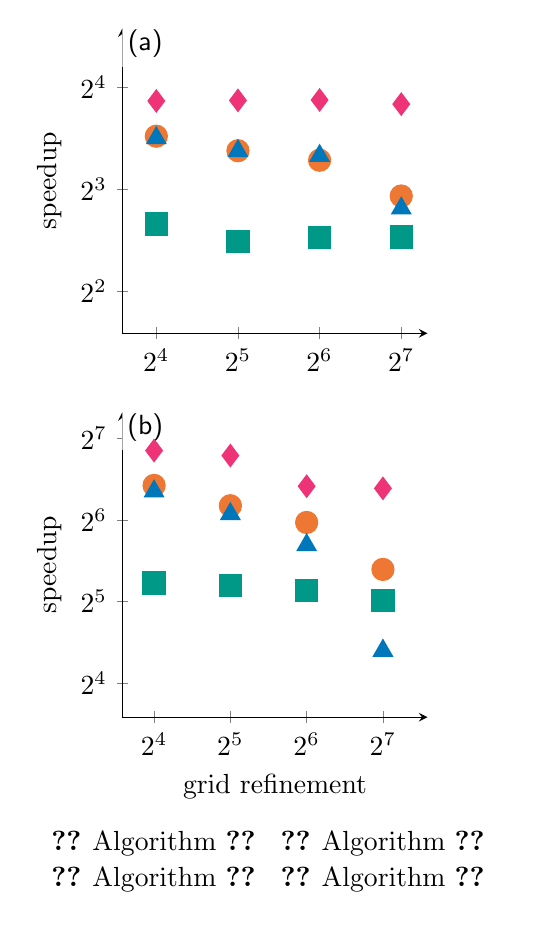
\begin{tikzpicture}
\begin{groupplot}[
    group style={group name=dep, group size=1 by 2},
    width=0.45\textwidth
]
\nextgroupplot[
        xmin=12,
        xmax=160,
        xmode=log,
        log basis x=2,
        ymin=3,
        ymax=24,
        ymode=log,
        log basis y=2,
        log origin=infty,
        ytick={2, 4, 8, 16},
        width=0.45\textwidth,
        height=0.45\textwidth,
        axis lines=center,
        ylabel={speedup},
        xlabel near ticks,
        ylabel near ticks
    ]
    
    \addplot+[only marks, mark=diamond*, color=tol/vibrant/magenta, mark options={scale=2, fill=tol/vibrant/magenta}] coordinates {%
        (16 , {1.44570/0.09890})
        (32 , {1.45665/0.09928})
        (64 , {1.46783/0.09974})
        (128, {1.51988/0.10624})
    }; \label{plot:grid-dep-interp};
    \addplot+[only marks, mark=square*, color=tol/vibrant/teal, mark options={scale=2, fill=tol/vibrant/teal}] coordinates {%
        (16 , {1.47196/0.23282})
        (32 , {1.48014/0.26431})
        (64 , {1.48519/0.25783})
        (128, {1.53801/0.26590})
    }; \label{plot:grid-dep-spread};
    \addplot+[only marks, mark=*, color=tol/vibrant/orange, mark options={scale=2, fill=tol/vibrant/orange}] coordinates {%
        (16 , {1.47196/0.12803})
        (32 , {1.48014/0.14213})
        (64 , {1.48519/0.15215})
        (128, {1.53801/0.20107})
    }; \label{plot:grid-dep-pa};
    \addplot+[only marks, mark=triangle*, color=tol/vibrant/blue, mark options={scale=2, fill=tol/vibrant/blue}] coordinates {%
        (16 , {1.47196/0.12965})
        (32 , {1.48014/0.14242})
        (64 , {1.48519/0.14766})
        (128, {1.53801/0.21874})
    }; \label{plot:grid-dep-otf};
    \node [fill=white] at (rel axis cs: 0.075, 0.95) {\sffamily(a)};
\nextgroupplot[
    xmin=12,
    xmax=192,
    xmode=log,
    log basis x=2,
    ymin=12,
    ymax=160,
    ymode=log,
    log basis y=2,
    log origin=infty,
    ytick={16, 32, 64, 128},
    width=0.45\textwidth,
    height=0.45\textwidth,
    axis lines=center,
    xlabel={grid refinement},
    ylabel={speedup},
    xlabel near ticks,
    ylabel near ticks
]
    \addplot+[only marks, mark=diamond*, color=tol/vibrant/magenta, mark options={scale=2, fill=tol/vibrant/magenta}] coordinates {%
        (16 , {1.44570/0.01253})
        (32 , {1.45665/0.01317})
        (64 , {1.46783/0.01722})
        (128, {1.51988/0.01816})
    };
    \addplot+[only marks, mark=square*, color=tol/vibrant/teal, mark options={scale=2, fill=tol/vibrant/teal}] coordinates {%
        (16 , {1.47196/0.03930})
        (32 , {1.48014/0.04020})
        (64 , {1.48519/0.04215})
        (128, {1.53801/0.04755})
    };
    \addplot+[only marks, mark=*, color=tol/vibrant/orange, mark options={scale=2, fill=tol/vibrant/orange}] coordinates {%
        (16 , {1.47196/0.01715})
        (32 , {1.48014/0.02049})
        (64 , {1.48519/0.02370})
        (128, {1.53801/0.03656})
    };
    \addplot+[only marks, mark=triangle*, color=tol/vibrant/blue, mark options={scale=2, fill=tol/vibrant/blue}] coordinates {%
        (16 , {1.47196/0.01804})
        (32 , {1.48014/0.02198})
        (64 , {1.48519/0.02873})
        (128, {1.53801/0.07288})
    };
    \node [fill=white] at (rel axis cs: 0.075, 0.95) {\sffamily(b)};
\end{groupplot}
\path (dep c1r2.south west|-current bounding box.south)--
coordinate(legendpos) (dep c1r2.south east|-current bounding box.south);
\matrix[
    matrix of nodes,
    anchor=north,
    inner sep=0.2em,
    %draw
  ]at([yshift=-1ex]legendpos)
  {
    \ref{plot:grid-dep-interp}& Algorithm \ref{algo:par-interp}&[5pt]
    \ref{plot:grid-dep-spread}& Algorithm \ref{algo:par-spread}&[5pt] \\
    \ref{plot:grid-dep-pa}& Algorithm \ref{algo:pa-spread}&[5pt]
    \ref{plot:grid-dep-otf}& Algorithm \ref{algo:otf-spread}\\};
\end{tikzpicture}
\caption{%
Speedup of Algorithm \ref{algo:par-interp} (interpolation) and Algorithms
\ref{algo:par-spread}--\ref{algo:otf-spread} (spreading) compared to their serial
counterparts on $2^{16}$ randomly placed IB points for different grid refinements on (a)
16 CPUs and (b) the GPU. 
}
\label{fig:grid-dependence}
\end{figure}

The speedup for these schemes is illustrated in Figure \ref{fig:grid-dependence}.
Algorithm \ref{algo:par-interp} is independent of the fluid grid, as expected. Any grid
dependence introduced by the sort and reduce steps of Algorithm \ref{algo:par-spread} is
not obvious for the grids presented. On the other hand, the degradation of speedup for
the sweep-fused Algorithms \ref{algo:pa-spread} and \ref{algo:otf-spread} is apparent for
finer grids. For small problems with $128^3$ or fewer grid points, one gets better
performance from the sweep-fused variants, with the exception of Algorithm
\ref{algo:otf-spread} on the GPU. This can be attributed to the slower allocation of the
buffer for a finer grid. For problems where the grid has $256^3$ or more grid points, we
expect Algorithm \ref{algo:par-spread} to be the fastest choice for spreading. Because
our fluid solver fits in GPU memory only for fewer than $128^3$ grid points, for the
remainder of this work we consider only a grid with a grid refinement of 64 ($h =
0.25\um$). We can imagine using this algorithm on a less capable device with more limited
memory, so we restrict ourselves to Algorithm \ref{algo:otf-spread} for spreading,
computing $\bufsz=8$ values per sweep, to minimize the lifetime of the buffer used in
spreading while still enjoying the benefit of using the buffer.

% vim: cc=90 tw=89

\subsubsection{Strong scaling}
It is commonly the case that we wish to employ parallelization to improve 
runtimes for a problem of interest. To illustrate this improvement, we now
consider how runtime varies for the test problem with $n=2^{16}$ IB points, a
grid refinement of 64 (grid size $h=0.25\um$), and Algorithm
\ref{algo:otf-spread} with different numbers of threads. We use up to 32
threads on the CPU and 64--4096 threads on the GPU. For a fixed problem, we
ideally wish to see the runtime using $2p$ threads to be half of that using
$p$ threads. In other words, the ideal speedup using twice as many threads is
2.


%\begin{table}[h]
%\begin{center}
%\bgroup
%\renewcommand{\arraystretch}{1.7}
%\begin{tabular}{cccc}
%                                                                                  \toprule
%    $p$  & device & \titletable{interpolate}{2000} & \titletable{spread}{1000} \\ \midrule
%         & CPU    & $1.30763 \pm 0.01795$          & $1.33840 \pm 0.01221$     \\
%    1    & CPU    & $1.30437 \pm 0.00986$          & $1.51528 \pm 0.02790$     \\
%    2    & CPU    & $0.67160 \pm 0.00605$          & $0.80398 \pm 0.02135$     \\
%    4    & CPU    & $0.35833 \pm 0.00284$          & $0.44432 \pm 0.01592$     \\
%    8    & CPU    & $0.21166 \pm 0.00773$          & $0.28799 \pm 0.04476$     \\
%    16   & CPU    & $0.10044 \pm 0.00258$          & $0.15393 \pm 0.01553$     \\
%    32   & CPU    & $0.07411 \pm 0.00068$          & $0.12394 \pm 0.01759$     \\
%    64   & GPU    & $0.80977 \pm 0.00478$          & $0.96698 \pm 0.00047$     \\
%    128  & GPU    & $0.43929 \pm 0.00352$          & $0.49359 \pm 0.00064$     \\
%    256  & GPU    & $0.22434 \pm 0.00223$          & $0.26208 \pm 0.00145$     \\
%    512  & GPU    & $0.11258 \pm 0.00150$          & $0.14286 \pm 0.00177$     \\
%    1024 & GPU    & $0.05681 \pm 0.00097$          & $0.08252 \pm 0.00150$     \\
%    2048 & GPU    & $0.03074 \pm 0.00071$          & $0.05351 \pm 0.00103$     \\
%    4096 & GPU    & $0.01689 \pm 0.00047$          & $0.03905 \pm 0.00093$     \\ \bottomrule
%\end{tabular}
%\egroup
%\caption{%
%    Strong scaling results for OTF and grid spacing $h = 0.5\um$ (a grid
%    refinement of 64) for $2^{16}$ randomly placed IB points in a
%    $16\um\times16\um\times16\um$ triply periodic domain. The first row
%    are reference values for serial Algorithms \ref{algo:par-interp} and
%    \ref{algo:serial-spread}.
%}
%\end{center}
%\end{table}

%1  & CPU & $1.29442 \pm 0.00359$ & $1.50377 \pm 0.00234$
%2  & CPU & $0.65481 \pm 0.00271$ & $0.92804 \pm 0.00147$
%4  & CPU & $0.34712 \pm 0.00166$ & $0.44697 \pm 0.00148$
%8  & CPU & $0.18004 \pm 0.00084$ & $0.24580 \pm 0.00082$
%16 & CPU & $0.09969 \pm 0.00075$ & $0.14895 \pm 0.00136$
%32 & CPU & $0.07371 \pm 0.00083$ & $0.12225 \pm 0.00143$

\begin{figure}[h]
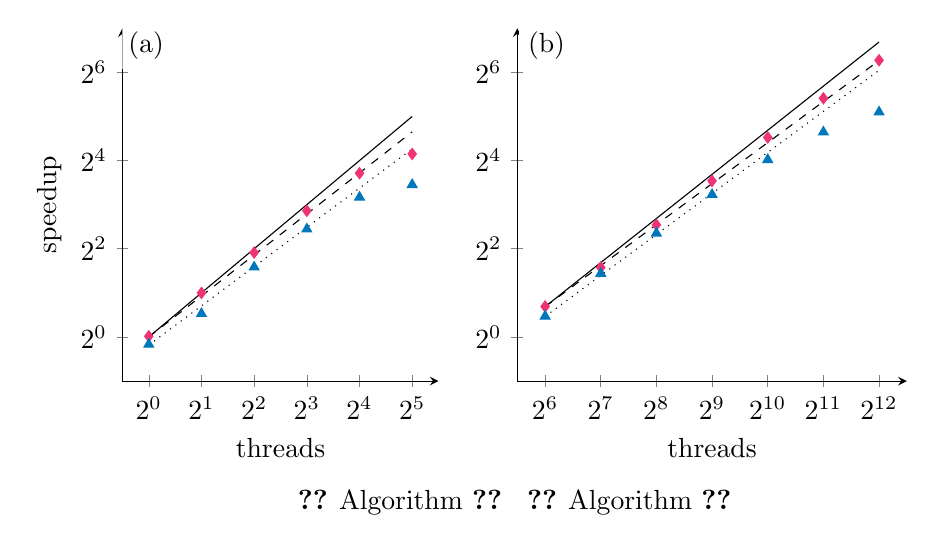
\begin{tikzpicture}
\begin{groupplot}[
    group style={group name=unst-strong, group size=2 by 1},
]
\nextgroupplot[
        xmin=0.70710678118,  % approx. 1/√2
        xmax=45.2548339959,  % approx 32√2
        xmode=log,
        log basis x=2,
        ymode=log,
        ymin=0.5,
        ymax=128,
        log basis y=2,
        log origin=infty,
        width=0.46153846153\textwidth,
        height=0.5\textwidth,
        axis lines=center,
        xlabel={threads},
        ylabel={speedup},
        xlabel near ticks,
        ylabel near ticks,
        xtick={1, 2, 4, 8, 16, 32},
        ytick={1, 4, 16, 64},
        legend style={at={(0.5, 0.9)}, anchor=center, draw=none,
                      /tikz/every even column/.append style={column sep=5pt}},
        legend cell align={left},
        legend columns=1
    ]
    \addplot+[only marks, mark=diamond*, color=tol/vibrant/magenta, mark options={fill=tol/vibrant/magenta}] coordinates {%
        (1 , {1.30763/1.29442})
        (2 , {1.30763/0.65481})
        (4 , {1.30763/0.34712})
        (8 , {1.30763/0.18004})
        (16, {1.30763/0.09969})
        (32, {1.30763/0.07371})
    }; \label{plot:unst-strong-interp}
    \addplot+[only marks, mark=triangle*, color=tol/vibrant/blue, mark options={fill=tol/vibrant/blue}] coordinates {%
        (1 , {1.33840/1.50377})
        (2 , {1.33840/0.92804})
        (4 , {1.33840/0.44697})
        (8 , {1.33840/0.24580})
        (16, {1.33840/0.14895})
        (32, {1.33840/0.12225})
    }; \label{plot:unst-strong-spread}
    \addplot+[no marks, dashed, black, domain=1:32] {x^0.93};
    \addplot+[no marks, dotted, black, domain=1:32] {0.88*x^0.89};
    \addplot+[no marks, black, domain=1:32] {x};
    \node[fill=white] at (rel axis cs: 0.075, 0.95) {(a)};
\nextgroupplot[
        xmin=45.2548339959,  % approx 32√2
        xmax=5792.61875148,  % approx 4096√2
        xmode=log,
        log basis x=2,
        ymode=log,
        ymin=0.5,
        ymax=128,
        log basis y=2,
        log origin=infty,
        width=0.53846153846\textwidth,
        height=0.5\textwidth,
        axis lines=center,
        xlabel={threads},
        xlabel near ticks,
        ylabel near ticks,
        ytick={1, 4, 16, 64},
        legend style={at={(0.5, 0.9)}, anchor=center, draw=none,
                      /tikz/every even column/.append style={column sep=5pt}},
        legend cell align={left},
        legend columns=1
    ]
    
    \addplot+[only marks, mark=diamond*, color=tol/vibrant/magenta, mark options={fill=tol/vibrant/magenta}] coordinates {%
        (64  , {1.30763/0.80977})
        (128 , {1.30763/0.43929})
        (256 , {1.30763/0.22434})
        (512 , {1.30763/0.11258})
        (1024, {1.30763/0.05681})
        (2048, {1.30763/0.03074})
        (4096, {1.30763/0.01689})
    };
    \addplot+[only marks, mark=triangle*, color=tol/vibrant/blue, mark options={fill=tol/vibrant/blue}] coordinates {%
        (64  , {1.33840/0.96698})
        (128 , {1.33840/0.49359})
        (256 , {1.33840/0.26208})
        (512 , {1.33840/0.14286})
        (1024, {1.33840/0.08252})
        (2048, {1.33840/0.05351})
        (4096, {1.33840/0.03905})
    };
    \addplot+[no marks, dashed, black, domain=64:4096] {1.61*(x/64)^0.93};
    \addplot+[no marks, dotted, black, domain=64:4096] {1.38*(x/64)^0.93};
    \addplot+[no marks, black, domain=64:4096] {1.61*x/64};
    \node[fill=white] at (rel axis cs: 0.075, 0.95) {(b)};
\end{groupplot}
\path (unst-strong c1r1.south west|-current bounding box.south)--
coordinate(legendpos) (unst-strong c2r1.south east|-current bounding box.south);
\matrix[
    matrix of nodes,
    anchor=north,
    inner sep=0.2em,
    %draw
  ]at([yshift=-1ex]legendpos)
  {
    \ref{plot:unst-strong-interp}& Algorithm \ref{algo:par-interp}&[5pt]
    \ref{plot:unst-strong-spread}& Algorithm \ref{algo:otf-spread}\\};
\end{tikzpicture}
\caption{%
    Strong scaling results for Algorithm \ref{algo:otf-spread} and grid spacing
    $h = 0.5\um$ (a grid refinement of 64) for $2^{16}$ randomly placed IB
    points in a $16\um\times16\um\times16\um$ triply periodic domain for
    (a) 1-32 CPU cores, and (b) 64-4096 threads on the GPU. Speedup is measured
    relative to serial Algorithms \ref{algo:par-interp} and
    \ref{algo:serial-spread}. The solid black lines show the trendline for
    ideal speedup. The dashed or dotted lines give the initial trend for
    interpolation and spreading, respectively.
}
\label{fig:unstructured-strong}
\end{figure}

Figure \ref{fig:unstructured-strong} shows the results of these tests. Speedup
is measured relative to the serial interpolation and spread implementations.
The trendlines estimate that increasing computing resources by a factor of two
decreases runtime by a factor or about 1.91 for CPU and GPU interpolation and
by a factor of about 1.85 for CPU spread.  It is not trivial to limit the
number of threads used by {\thrust} for work done on the GPU, so the key-value
sort and segmented reduce use as many threads as {\thrust} decides is prudent.
While the trendline indicates a decrease in runtime by a factor of 1.91 as
well, this is merely an approximation.  

Parallel CPU interpolate using a single processor is identical to the serial
CPU interpolate, so the CPU interpolate passes through $(1,\,1)$. The same is
not true of the parallel spread using a single processor compared to serial
spread. Because of the additional sort step in the parallel spread algorithm,
single-threaded Algorithm \ref{algo:par-spread} is about 12\% slower than its
serial counterpart. The CPU code also enjoys the benefit of using vector
registers for some of the computation. The GPU requires 64 threads to match
the speed of a single CPU core. Based on the trendline in Figure
\ref{fig:unstructured-strong} and the speedup for grid refinement shown in
Figure \ref{fig:grid-dependence}, we see that the GPU attains a speedup of
approximately 5.25$\times$ compared to 32 CPU processors, and uses
approximately 4480 threads, where the kernel reaches the limit on register
memory.

%\bgroup\color{red}
%Interestingly, even at 4096 threads,  parallel interpolate on the GPU shows no
%indication of plateauing. The final data point for that curve shows a speedup
%of approximately 77$\times$. Figure \ref{fig:grid-dependence}, on the other
%hand, shows that the maximum speedup we can expect for this problem is 
%approximately 84$\times$, which the trendline predicts will occur at
%approximately 4480 threads. Thus, we can expect the plateau for parallel
%interpolate on the GPU to be very abrupt. The parallelization may be limited
%by the GPUs register file size, 256KB, where each thread is using 14 32-bit
%registers.
%\egroup

Overall, trends for the CPU and GPU are very similar. The plateauing of the
CPU curves may not be the limitations of the algorithm for the CPU. Despite
having 48 cores, the test using 32 cores did not utilize them at full capacity.
Using fewer cores, on the other hand, was able to maintain full utilization
for the duration of the test. If not for having a comparatively limited number
of CPU cores, we expect to see the CPU trend continue. Because of these
similarities, we will restrict ourselves to the GPU, but expect any conclusions
to hold for the CPU as well.

\subsubsection{Weak scaling}\label{sec:unst-weak}
In contrast, with improved computing resources, we may wish to solve bigger
problems. The ideal parallel algorithm solves a problem with $p$ threads in the
same time as it solves a twice bigger problem with $2p$ threads. Here, we place
between $2^{16}$ and $2^{19}$ points randomly in the domain. We increase the
number of threads proportionally, between 128 and 1024.  

\begin{table}
    \begin{center}
        \begingroup
        \setlength{\tabcolsep}{9pt}
        \renewcommand{\arraystretch}{1.5}
        \begin{tabular}{ccccc}
                                                                                              \toprule
            $p$  & $n$      & \titletable{interpolate}{20000} & \titletable{spread}{10000} \\ \midrule
            128  & $2^{16}$ & $0.43930 \pm 0.00019$           & $0.47632 \pm 0.00142$      \\
            256  & $2^{17}$ & $0.44918 \pm 0.00056$           & $0.46503 \pm 0.00026$      \\
            512  & $2^{18}$ & $0.45072 \pm 0.00061$           & $0.44533 \pm 0.00028$      \\
            1024 & $2^{19}$ & $0.45442 \pm 0.00049$           & $0.43561 \pm 0.00024$      \\ \bottomrule
        \end{tabular}
        \endgroup
    \end{center}
    \caption{%
        Weak scaling results for $p$ threads and $n$ randomly placed IB points
        in a $16\um\times16\um\times16\um$ triply periodic domain with
        $h=0.5\um$ on the GPU. Times are reported in seconds. $N$ is the number
        of samples taken.
    }
    \label{tab:unstructured-weak}
\end{table}

Table \ref{tab:unstructured-weak} lists runtimes for increasing threads and
problem size on the GPU. Interpolate scales nearly perfectly with a difference
of $15\ms$ (\textasciitilde3\%) increase between the problem with 128 threads
and $2^{16}$ IB points and that with 1024 threads and $2^{19}$ points. Spread,
on the other hand, decreases in time as the problem size increases. This
speedup is artificial, and should not be expected in general. In the $n=2^{16}$
case, there is 1 point for every 4 grid cells, on average. When $n=2^{19}$,
the density increases to 2 for every grid cell. As a result, it becomes
increasingly unlikely to find a cell containing no IB points. This means that
writing the values to the output vector(s) becomes increasingly coalesced,
which, in turn, reduces the number of writes to global memory and vastly
improves the speed of the write overall. Typical use of the IB method does not
have IB points in every grid cell, but the recommendations that IB points on
connected structures be spaced $0.5h$--$h$ apart typically yields 1--4 IB
points in each occupied grid cell. We now consider a more typical use of the IB
method.


\subsection{Structured IB point results}

In this section, we replace the randomly-placed IB points with points sampled
on the surface of a red blood cell (RBC). For a grid spacing of $h=0.5\um$, we
may use $n_d = 864$ data sites, which spaces points approximately $0.8h$ apart,
and $n_s = 8832$ sample sites, which spaces points approximately $0.5h$ apart,
per RBC. In other words, we interpolate the fluid velocity to 864 points per
RBC while forces are computed at and spread from 8832 points per RBC. These
points, and those for other grids, are generated by the \texttt{KernelNode}
library. Here, we invoke the fluid solver, so that as the RBC deforms, the
force it imparts on the fluid will affect the fluid velocity. The RBC is
modeled as an elastic structure, obeying the Skalak constitutive law
[@Skalak:XXX] with shear modulus $2.5\times10^{-3}\si{dyn\per\centi\meter}$ and
bulk modulus $2.5\times10^{-1}\si{dyn\per\centi\meter}$. The timestep required
for stability in this test is $k=1\times 10^{-7}\si{\second}$.

We begin by confirming the convergence of the solution.

\subsubsection{Convergence study}
To test the convergence of the fluid solver and cell representation, consider 
an object that obeys Skalak's law with the coefficients given above and is
spherical at rest. Deform the object from its rest configuration by stretching
it by a factor of $1.1$ in the $z$ direction and compressing it by a factor of
$1.1$ in the $y$ direction to maintain a fixed volume. For this test, $\shear$
is zero, so the fluid velocity is intially zero, and the object tends toward
its rest configuration over the course of simulation. We allow the object to
relax for $16\us$, and compare errors generated by successive grid refinements
of 16, 32, 64, and 128 points per $16\um$. For each grid, we use a fixed set of
$n_d=625$ data sites, sampled approximately uniformly on the surface of the
sphere, and choose $n_s$ so that sample sites are approximately uniform and
roughly $h/1.1$ apart, so that sample sites are roughly $h$ apart initially.
For $h=1\um$, $n_s=220$, and a refinement by a factor of 2 increases $n_s$ by a
factor of 4, for a maximum number of 14080 sample sites for these tests. A thin
interface which generates a force will cause a jump in the normal stress across
the interface, which the IB method may not recover. We therefore anticipate
first order convergence for the fluid velocity and data site positions.

\begin{table*}[ht]
    \begin{center}
        \begingroup
        \setlength{\tabcolsep}{9pt}
        \renewcommand{\arraystretch}{1.5}
        \begin{tabular}{cc|cc|cc}
                                                                                                                    \\ \toprule
            $h$ ($\um$) & $k$ ($\us$) & $\|\u_h-\u_{0.5h}\|_2$ & order   & $\|\u_h-\u_{0.5h}\|_{\infty}$ & order    \\ \midrule
            $1.00$      & $1.6$       & $2.2274\times10^{-2}$  &         & $7.4187\times10^{-2}$         &          \\
            $0.50$      & $0.4$       & $4.3280\times10^{-4}$  & 5.71513 & $1.9083\times10^{-3}$         & 5.28079  \\
            $0.25$      & $0.1$       & $1.4684\times10^{-4}$  & 1.55951 & $1.0847\times10^{-3}$         & 0.81497  \\ \bottomrule
        \end{tabular}
        \endgroup
    \end{center}
    \caption{%
Convergence of the fluid velocity for a deformed sphere returning to its rest
configuration in a $16\um\times16\um\times16\um$ triply periodic domain at
$t=160\us$. The finest grid, with $h=0.125\um$ uses timestep $k=0.025\us$.
    }
    \label{tab:u-convergence}
\end{table*}

\begin{table*}[ht]
    \begin{center}
        \begingroup
        \setlength{\tabcolsep}{9pt}
        \renewcommand{\arraystretch}{1.5}
        \begin{tabular}{cc|cc|cc}
                                                                                                             \\ \toprule
            $h$ ($\um$) & $n_s$ & $\|\X_h-\X_{0.5h}\|_2$ & order   & $\|\X_h-\X_{0.5h}\|_{\infty}$ & order   \\ \midrule
            $1.00$      & 220   & $2.9611\times10^{-3}$  &         & $4.7812\times10^{-3}$         &         \\
            $0.50$      & 880   & $7.2997\times10^{-4}$  & 2.02020 & $1.1687\times10^{-3}$         & 2.03253 \\
            $0.25$      & 3520  & $3.5909\times10^{-4}$  & 1.02351 & $6.0956\times10^{-4}$         & 0.93902 \\ \bottomrule
        \end{tabular}
        \endgroup
    \end{center}
    \caption{%
Convergence of data sites for a deformed sphere returning to its rest
configuration in a $16\um\times16\um\times16\um$ triply periodic domain at
$t=16\us$. For each grid, we track 625 data sites on the sphere. The finest
grid, with $h = 0.125\um$ used $n_s=14080$ sample sites.
    }
    \label{tab:x-convergence}
\end{table*}

Tables \ref{tab:u-convergence} and \ref{tab:x-convergence} show the convergence
of fluid velocity and data sites, respectively. To compute errors in the fluid
velocity, we construct a cubic spline from the velocities on the finer grid
and evaluate the spline at the grid points of the coarser grid. Each of the
interfaces is constructed with the same number of data sites, so the
coordinates from one simulation to another can be compared directly. We recover
approximately first order convergence for both fluid velocity and data sites
positions. Having established asymptotic convergence of our IB solver, we
continue by performing scaling tests with RBCs.

\subsubsection{Strong scaling}

We again wish to see how these algorithms can help speed up the runtime of
a fixed problem. Here, we consider tests with a single RBC and with 4 RBCs.
To construct the RBCs, we now use $n_d=864$ data sites, for an initial data
site spacing of approximately $0.8h$, and $n_s=8832$ sample sites per cell, for
an initial sample site spacing for approximately $0.25h$. We use a timestep of
$k=0.1\us$ to simulate the motion of the cells for $1\ms$.

%\begin{table}
%    \begin{center}
%        \begingroup
%        \setlength{\tabcolsep}{9pt}
%        \renewcommand{\arraystretch}{1.5}
%        \begin{tabular}{ccccc}
%            $p$  & cells & \titletable{interpolate}{20000} & \titletable{spread}{10000} \\ \hline
%%            1    & 1     & $0.47633 \pm 0.00024$           & $4.58460 \pm 0.00821$      \\
%%            2    & 1     & $0.26608 \pm 0.00146$           & $2.59113 \pm 0.00567$      \\
%%            4    & 1     & $0.14505 \pm 0.00080$           & $1.44780 \pm 0.00353$      \\
%%            8    & 1     & $0.07593 \pm 0.00031$           & $0.76037 \pm 0.00229$      \\
%%            16   & 1     & $0.04010 \pm 0.00009$           & $0.40348 \pm 0.00137$      \\
%%            32   & 1     & $0.02037 \pm 0.00007$           & $0.22602 \pm 0.00105$      \\
%            64   & 1     & $0.01080 \pm 0.00004$           & $0.11888 \pm 0.00055$      \\
%            128  & 1     & $0.00586 \pm 0.00002$           & $0.06535 \pm 0.00023$      \\
%            256  & 1     & $0.00341 \pm 0.00002$           & $0.03912 \pm 0.00012$      \\
%            512  & 1     & $0.00179 \pm 0.00001$           & $0.02649 \pm 0.00014$      \\
%            1024 & 1     & $0.00093 \pm 0.00001$           & $0.01924 \pm 0.00011$      \\
%            2048 & 1     & $0.00094 \pm 0.00001$           & $0.01627 \pm 0.00012$      \\
%            4096 & 1     & $0.00093 \pm 0.00001$           & $0.01455 \pm 0.00009$%      \\
%%            8192 & 1     & $0.00094 \pm 0.00001$           & $0.01413 \pm 0.00010$
%        \end{tabular}
%        \endgroup
%    \end{center}
%    \caption{%
%        Results of strong scaling tests for IB spread and interpolate.
%        Reported values are in seconds.
%    }
%\end{table}

\begin{figure}[ht]
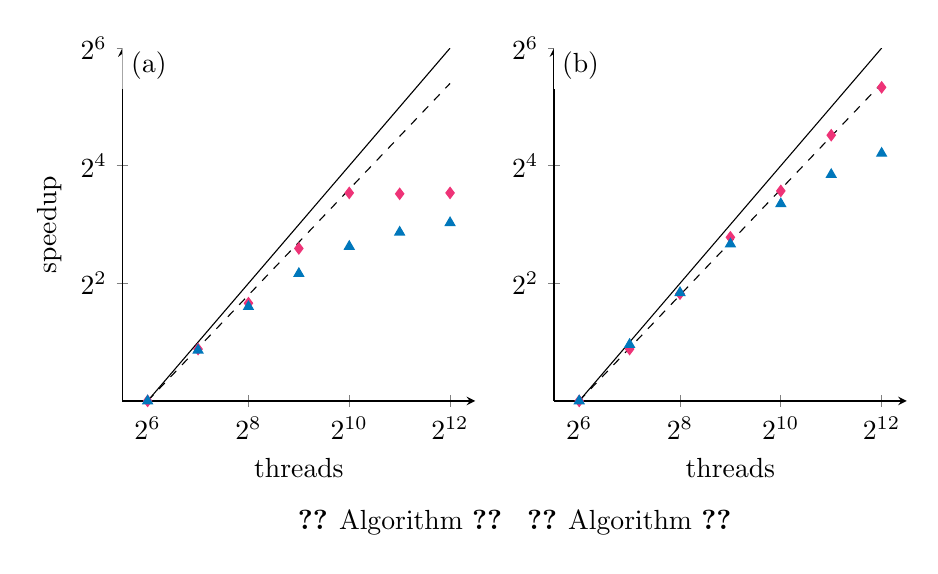
\begin{tikzpicture}
\begin{groupplot}[
    group style={group name=rbc-strong, group size=2 by 1},
    height=0.5\textwidth,
    width=0.5\textwidth
]
\nextgroupplot[
        xmode=log,
        xmin=45.2548339959,
        xmax=5792.61875148,
        log basis x=2,
        ymode=log,
        ymax=64,
        log basis y=2,
        log origin=infty,
        width=0.5\textwidth,
        height=0.5\textwidth,
        axis lines=center,
        xlabel={threads},
        ylabel={speedup},
        xlabel near ticks,
        ylabel near ticks,
        legend style={at={(0.8, 0.2)}, anchor=center},
        legend cell align={left}
]
    \addplot+[only marks, mark=diamond*, color=tol/vibrant/magenta, mark options={fill=tol/vibrant/magenta}] coordinates {%
        (64  , {0.01080/0.01080})
        (128 , {0.01080/0.00586})
        (256 , {0.01080/0.00341})
        (512 , {0.01080/0.00179})
        (1024, {0.01080/0.00093})
        (2048, {0.01080/0.00094})
        (4096, {0.01080/0.00093})
    }; \label{plot:rbc-interp}
    \addplot+[only marks, mark=triangle*, color=tol/vibrant/blue, mark options={fill=tol/vibrant/blue}] coordinates {%
        (64  , {0.11888/0.11888})
        (128 , {0.11888/0.06535})
        (256 , {0.11888/0.03912})
        (512 , {0.11888/0.02649})
        (1024, {0.11888/0.01924})
        (2048, {0.11888/0.01627})
        (4096, {0.11888/0.01455})
    }; \label{plot:rbc-spread}
    \addplot+[no marks, dashed, black, domain=64:4096] {(x/64)^0.9};
    \addplot+[no marks, black, domain=64:4096] {(x/64)};
    \node [fill=white] at (rel axis cs: 0.075, 0.95) {(a)};
\nextgroupplot[
        xmode=log,
        xmin=45.2548339959,
        xmax=5792.61875148,
        log basis x=2,
        ymode=log,
        ymax=64,
        log basis y=2,
        log origin=infty,
        width=0.5\textwidth,
        height=0.5\textwidth,
        axis lines=center,
        xlabel={threads},
        xlabel near ticks,
        ylabel near ticks,
        legend style={at={(0.8, 0.2)}, anchor=center},
        legend cell align={left}
    ]
    \addplot+[only marks, mark=diamond*, color=tol/vibrant/magenta, mark options={fill=tol/vibrant/magenta}] coordinates {%
        (64  , {0.04150/0.04150})
        (128 , {0.04150/0.02251})
        (256 , {0.04150/0.01172})
        (512 , {0.04150/0.00603})
        (1024, {0.04150/0.00349})
        (2048, {0.04150/0.00181})
        (4096, {0.04150/0.00103})
    };
    \addplot+[only marks, mark=triangle*, color=tol/vibrant/blue, mark options={fill=tol/vibrant/blue}] coordinates {%
        (64  , {0.40148/0.40148})
        (128 , {0.40148/0.20628})
        (256 , {0.40148/0.11208})
        (512 , {0.40148/0.06313})
        (1024, {0.40148/0.03931})
        (2048, {0.40148/0.02785})
        (4096, {0.40148/0.02168})
    };
    \addplot+[no marks, dashed, black, domain=64:4096] {(x/64)^0.9};
    \addplot+[no marks, black, domain=64:4096] {(x/64)};
    \node [fill=white] at (rel axis cs: 0.075, 0.95) {(b)};
\end{groupplot}
\path (rbc-strong c1r1.south west|-current bounding box.south)--
coordinate(legendpos) (rbc-strong c2r1.south east|-current bounding box.south);
\matrix[
    matrix of nodes,
    anchor=north,
    inner sep=0.2em,
    %draw
  ]at([yshift=-1ex]legendpos)
  {
      \ref{plot:rbc-interp}& Algorithm \ref{algo:par-interp}&[5pt]
      \ref{plot:rbc-spread}& Algorithm \ref{algo:otf-spread} \\};
\end{tikzpicture}
\caption{%
    Speedup of Algorithms \ref{algo:par-interp} and \ref{algo:otf-spread} with
    increasing numbers of threads compared to 64 threads on the GPU for (a) 1
    and (b) 4 RBCs. Speedup is measured relative to the time taken for each
    algorithm using 64 threads on the GPU. Dashed lines indicate trends, and
    solid lines indicate ideal scaling.
}
\label{fig:str-strong}
\end{figure}

Figure \ref{fig:str-strong} shows the speedup observed with increasing threads
for 1 and 4 RBCs for 64--4096 threads on the GPU. We again see that the initial
speedup for interpolation is nearly linear with increased threads. In subfigure
(a), there is a sharp plateau that corresponds to every data site having its
own thread. In other words, there are more threads than there is work to be
done, since we track only 864 data sites for a single RBC. Subfigure (b), on
the other hand, has 3456 data sites, so the trend continues for 512--4096
threads. In this case, we expect this graph to plateau beyond 4096, as each
data site already has its own thread. However, we do not expect for the trend
to continue with more cells, as the presumed maximum number of threads for
interpolation is 4480, as discussed in Section [@sec:grid-dependence]. 
Comparing subfigure (a) to (b), for spread, we see that the speedup is also
dependent on the amount of work. This indicates that, as with interpolation,
the maximum speedup for spread is limited by hardware, rather than being a
limitation of the algorithm.

The trendlines for these tests indicate that increasing computing resources
by a factor of two decreases runtime by a factor of about 1.87 for these
algorithms. Again, this is merely an approximation as the sort and reduction
steps of the spread algorithm are provided by {\thrust}, and therefore are
not limited to the listed number of threads. The similarity between the result
of the tests with RBCs and with randomly placed points indicates that the
distribution of points does not have a marked impact on the efficacy of the
parallelization for a fixed problem. We now see if the same holds for weak
scaling tests.


%\begin{table}
%    \begin{center}
%        \begingroup
%        \setlength{\tabcolsep}{9pt}
%        \renewcommand{\arraystretch}{1.5}
%        \begin{tabular}{ccccc}
%            $p$   & cells & \titletable{interpolate}{20000} & \titletable{spread}{10000} \\ \hline
%            64    & 4     & $0.04150 \pm 0.00013$           & $0.40148 \pm 0.00146$      \\
%            128   & 4     & $0.02251 \pm 0.00003$           & $0.20628 \pm 0.00060$      \\
%            256   & 4     & $0.01172 \pm 0.00002$           & $0.11208 \pm 0.00031$      \\
%            512   & 4     & $0.00603 \pm 0.00002$           & $0.06313 \pm 0.00014$      \\
%            1024  & 4     & $0.00349 \pm 0.00002$           & $0.03931 \pm 0.00011$      \\
%            2048  & 4     & $0.00181 \pm 0.00001$           & $0.02785 \pm 0.00011$      \\
%            4096  & 4     & $0.00103 \pm 0.00001$           & $0.02168 \pm 0.00009$
%        \end{tabular}
%        \endgroup
%    \end{center}
%    \caption{%
%        Results of strong scaling tests for IB spread and interpolate with
%        4 RBCs.
%        Reported values are in seconds.
%    }
%\end{table}

\subsubsection{Weak scaling}

To see how the algorithms scale given more computing resources, we increase the
number of cells in the domain and the number of threads proportionally. We
construct each cell with $n_d=864$ data sites and $n_s=8832$ sample sites, as
before. We place between 1 and 8 cells in the domain, while threads increase
from 64 to 512. Using a timestep of $k = 0.1\us$, we simulate the motion of
these cells for $1\ms$.

In Section \ref{sec:unst-weak}, we observe that, as a side-effect of increasing
point density per grid cell, runtime for spreading decreases as the number of
points and threads increases. Here, the cells are initially far enough part as
to not have any overlapping support points.  As a result, while individual grid
cells may contain several IB points, average point density is still low, so we
do not expect to see the same reduction in runtime as observed previously.

\begin{table}[t]
    \caption{%
Weak scaling results for interpolate and spreading for increasing numbers of
RBCs (cells column) and threads. Each RBC has $n_d = 864$ and $n_s = 8832$.
Average time per call is reported in seconds. $N$ is the number of samples
taken.}\label{tab:str-weak}
    \begin{center}
        \begingroup
        \setlength{\tabcolsep}{9pt}
        \renewcommand{\arraystretch}{1.5}
        \begin{tabular}{ccccc}
                                                                                          \toprule
            $p$ & cells & \titletable{interpolate}{20000} & \titletable{spread}{10000} \\ \midrule
            64  & 1     & $0.01079$                       & $0.11881$                  \\
            128 & 2     & $0.01165$                       & $0.11219$                  \\
            256 & 4     & $0.01171$                       & $0.11214$                  \\
            512 & 8     & $0.01199$                       & $0.11354$                  \\ \bottomrule
        \end{tabular}
        \endgroup
    \end{center}
\end{table}

Table \ref{tab:str-weak} shows the runtimes for increasing number of RBCs and
threads. We observe the near-perfect scaling we saw with random IB points. For
both interpolate and spread, we see that the runtimes are nearly constant: the
slowest and fastest times differ by less than $2\ms$ and $7\ms$, for
interpolation and spread, respectively. After an initial drop in runtime
between one RBC with 64 threads and two RBCs and 128 threads, runtimes even off
and begin to increase, in contrast with the results in Section
\ref{sec:unst-weak}.


\section{Summary}

We have presented a parallel algorithm for interpolation and introduced a novel parallel
algorithm for spreading forces from time-dependent interfaces in the immersed boundary
method. These algorithms have a runtime that is independent of the Eulerian grid. This
makes the parallelization useful for cases where IB points inhabit only a small
percentage of the Eulerian grid cells. We have also introduced two variants for spread
which trade off dependence on the Eulerian grid, in the form of a few vector adds and
memory allocation, for improved runtimes for small enough grids.

These algorithms exhibit nearly ideal scaling, on both the CPU and GPU, for problems of
fixed size and increasing number of threads, as well as for problems of increasing size
and number of threads.  We observed that on the GPU, larger problem sizes led to higher
speedup plateaus, indicating that larger problems on more capable hardware will achieve
even larger speedups than presented here.

% vim: cc=90 tw=89


%\begin{acknowledgements}
%\end{acknowledgements}


% Authors must disclose all relationships or interests that 
% could have direct or potential influence or impart bias on 
% the work: 
%

%\section*{Conflict of interest}


\bibliographystyle{spmpsci}      % mathematics and physical sciences
\end{document}
% end of file template.tex

